\documentclass[conference]{IEEEtran}
\IEEEoverridecommandlockouts

\usepackage{cite}
\usepackage{amsmath,amssymb,amsfonts}
\usepackage{algorithmic}
\usepackage{graphicx}
\usepackage{textcomp}
\usepackage{xcolor}
\usepackage{booktabs}
\usepackage{multirow}
\usepackage{url}
\usepackage{microtype}
\usepackage{subcaption}

\def\BibTeX{{\rm B\kern-.05em{\sc i\kern-.025em b}\kern-.08em
    T\kern-.1667em\lower.7ex\hbox{E}\kern-.125emX}}

\begin{document}

\title{Personalized Electrocardiographic and HRV Dynamics for Acute Stress Detection: A Leave-One-Subject-Out Benchmark and Bare-Metal Edge IoMT Implementation}

\author{\IEEEauthorblockN{Mukesh Yadav}
\IEEEauthorblockA{\textit{Department of Electronics and Communication Engineering (ECE)} \\
\textit{JSS Academy of Technical Education (JSSATEN)}\\
Noida, Uttar Pradesh, India \\
Email: mkpy06@gmail.com}
}

\maketitle

\begin{abstract}
Automated classification of acute psychological stress from non-invasive wearable electrocardiography (ECG) is a fundamental problem in physiological computing, affective state recognition, and wearable Internet of Medical Things (IoMT). A central barrier to cross-subject generalization is inter-individual baseline heterogeneity: resting heart rate and basal heart rate variability (HRV) metrics vary widely across individuals due to genetic, cardiorespiratory fitness, and circadian factors, causing uncalibrated global classifiers to degrade substantially on unseen subjects. Furthermore, resource constraints and telemetry-privacy vulnerabilities pose major roadblocks for edge-node wearable deployment. In this work, we present an end-to-end reproducible research pipeline benchmarked across all 15 subjects ($N=15$, 445 standardized 60-second windows) of the public Wearable Stress and Affect Detection (WESAD) dataset, paired with a bare-metal embedded microcontroller deployment. Single-lead chest ECG acquired at 700~Hz is conditioned via zero-phase 4th-order Butterworth filtering (0.5--40~Hz), followed by adaptive noise-floor peak prominence detection and physiological interval gating. A selected 8-feature representation capturing heart rate, time-domain variability, and robust spread metrics is transformed via subject-specific relative baseline calibration: $X^* = (X - B_s) / |B_s|$. Evaluated under strict 15-fold Leave-One-Subject-Out Cross-Validation (LOSO-CV), baseline-relative calibration elevates classification accuracy from 81.57\% to 92.36\% (+10.79\%) and stress F1-score from 73.03\% to 89.03\% (+16.00\%) over identical unnormalized baselines. At a calibrated decision threshold of $\tau = 0.35$, the primary model achieves an ROC-AUC of 0.9494, PR-AUC of 0.9467, sensitivity of 86.25\%, and specificity of 95.79\%. A comparative benchmark across six machine learning architectures demonstrates consistent generalization (ROC-AUC $>$ 0.937). Permutation importance and odds ratio analyses indicate that cardiac interval compression ($\Delta\text{MeanRR}$) and heart rate acceleration ($\Delta\text{MeanHR}$) are the primary contributors to the learned boundary. Translating this framework to physical hardware, we implement a bare-metal edge processing node on the ARM Cortex-M4 microcontroller (STM32G474RE, 16~MHz HSI). Real-time signal conditioning is executed via an on-chip 5-stage Direct Form II Transposed Biquad IIR filter executing in $\approx 1.87~\mu\text{s}$ per sample ($<$0.1\% CPU utilization at 350~Hz). To safeguard patient privacy against casual wire tapping, an on-chip 32-bit discrete chaotic stream scrambler (Marsaglia Xorshift32 + Golden Ratio Weyl sequence with Nonce-CBC diffusion) executes in $2.0~\mu\text{s}$ (32 clock cycles), elevating wire Shannon entropy to $H = 7.25\text{--}7.98\text{ bits/byte}$ while supporting bit-exact ($0.000000\text{ V}$) terminal descrambling. Continuous hardware-in-the-loop streaming over 15,000 packets demonstrates 100\% frame synchronization and zero CRC errors (100\% transmission reliability) across authorized monitoring and adversarial eavesdropper operating modes.
\end{abstract}

\begin{IEEEkeywords}
Wearable sensing, electrocardiography (ECG), heart rate variability (HRV), acute stress detection, baseline calibration, edge computing, STM32, ARM Cortex-M4, chaotic stream scrambling, IoMT security, WESAD.
\end{IEEEkeywords}

\section{Introduction}
Acute psychological stress triggers a complex neuroendocrine cascade governed by the sympathetic division of the autonomic nervous system (ANS). Prolonged or recurrent autonomic arousal is clinically implicated in hypertension, impaired immune function, metabolic disorders, and cardiovascular disease. Continuous, non-invasive physiological monitoring via wearable biomedical sensors offers unprecedented potential for early detection and closed-loop biofeedback interventions \cite{can2019continuous}.

Among non-invasive biosignals, the electrocardiogram (ECG) and its derivative Normal-to-Normal (NN) inter-beat intervals provide a sensitive, temporally dynamic window into cardiac autonomic regulation \cite{taskforce1996hrv}. However, machine learning models trained on raw, global heart rate variability (HRV) metrics consistently suffer from severe performance drops when deployed across novel individuals. This challenge stems from \textit{inter-individual baseline heterogeneity}: basal resting heart rates in healthy adults commonly range from 50 to 90 beats per minute (BPM), and basal autonomic tone varies substantially across individuals \cite{taskforce1996hrv, shaffer2017overview}. Consequently, a fixed global threshold (e.g., classifying stress whenever $\text{HR} > 80$~BPM) produces high false-positive rates for individuals with elevated resting heart rates and fails to detect acute stress in athletic individuals with resting bradycardia.

Beyond algorithmic generalization, deploying continuous physiological computing on wearable edge nodes presents severe cyber-physical challenges \cite{alturjman2020iomt, sugita2015mental}. Low-power microcontrollers possess limited SRAM and clock speeds, rendering heavy digital filtering and deep neural networks impractical. Furthermore, wireless/serial telemetry of raw physiological signals exposes sensitive biometric identity and autonomic health states to unauthorized physical eavesdropping.

To overcome these fundamental barriers, we present a personalized physiological framework evaluated under rigorous Leave-One-Subject-Out (LOSO) cross-validation on the public WESAD benchmark \cite{schmidt2018wesad}, coupled with a physical bare-metal ARM Cortex-M4 edge node implementation. The primary contributions of this work include:
\begin{enumerate}
    \item \textbf{Subject-Specific Relative Normalization:} We demonstrate that formulating features as fractional deviations relative to each subject's resting baseline ($X^* = (X - B_s) / |B_s|$) provides an empirical boost of +10.79\% in accuracy and +16.00\% in F1-score over identical unnormalized feature sets.
    \item \textbf{Rigorous 15-Fold LOSO Evaluation:} We benchmark the full 15-subject cohort ($N=15$) under strict label-isolated Leave-One-Subject-Out evaluation with unsupervised baseline calibration, preventing test-label exposure across folds and achieving 92.36\% accuracy and an ROC-AUC of 0.9494.
    \item \textbf{Comprehensive ML \& Explainability Suite:} We benchmark six canonical machine learning paradigms and conduct a 30-repeat permutation importance analysis per fold ($15 \times 30 = 450$ trials per feature) alongside standardized odds ratios to quantitatively interpret the physiological decision boundary.
    \item \textbf{Bare-Metal Edge DSP on STM32G474RE:} We implement and flash a real-time signal conditioning engine on an ARM Cortex-M4 microcontroller featuring a 5-stage Direct Form II Transposed Biquad IIR filter ($f_s = 350$~Hz) consuming only $1.87~\mu\text{s}$ per sample ($<$0.1\% CPU utilization at 16~MHz).
    \item \textbf{On-Chip Discrete Chaotic Stream Scrambling \& Obfuscation:} We deploy an ultra-lightweight 32-bit discrete chaotic stream scrambler ($2.0~\mu\text{s}$, 32 cycles) that elevates wire Shannon entropy to $H = 7.25\text{--}7.98$~bits/byte to protect cardiac telemetry against unauthorized wire eavesdropping, verified via a synchronized dual-mode monitoring/adversarial dashboard across 15,000+ packets with zero CRC frame drops.
\end{enumerate}

\section{Related Work \& Benchmarks}
Physiological stress detection has historically relied on multimodal laboratory protocols combining ECG, electrodermal activity (EDA), respiration, and surface electromyography \cite{healey2005detecting, plarre2011continuous, sugita2015mental}. In 2018, Schmidt \textit{et al.} introduced the Wearable Stress and Affect Detection (WESAD) dataset \cite{schmidt2018wesad}, which has become a widely adopted benchmark for wearable affective computing.

In their seminal benchmark study, Schmidt \textit{et al.} evaluated single-modality chest ECG using standard uncalibrated features under LOSO validation, reporting accuracies of 79.03\% with Decision Trees and 83.84\% with Random Forests (F1-scores of 71.43\% and 75.12\%, respectively). While multimodal combinations (combining ECG with EDA and respiration) yielded higher accuracies, relying purely on single-lead ECG remains highly desirable due to its low hardware cost, high user acceptance, and integration into commercial chest straps and smart patches. Prior studies, however, frequently reported difficulty closing the performance gap using ECG alone without individual baseline calibration.

In parallel, the rise of the Internet of Medical Things (IoMT) has driven demand for edge-native biomedical intelligence \cite{alturjman2020iomt}. Real-time wearable nodes require embedded digital filtering \cite{oppenheim1999discrete, elgendi2013fast} and low-latency feature extraction to minimize power-intensive wireless transmissions. Simultaneously, safeguarding physiological telemetry against unauthenticated wiretapping benefits from lightweight telemetry obfuscation primitives with minimal computational overhead \cite{marsaglia2003xorshift}, a challenge directly tackled in our physical hardware pipeline.

\section{Dataset \& Experimental Protocol}
\subsection{WESAD Experimental Protocol}
We evaluated our methodology on the public WESAD dataset \cite{schmidt2018wesad}. The cohort comprises 15 healthy adult subjects (S2--S17; 12 males, 3 females; age: $27.5 \pm 2.4$ years). Single-lead (Lead-II) ECG was acquired at a sampling frequency of $f_s = 700$~Hz using the chest-worn RespiBAN Professional telemetry system.

The data acquisition followed a standardized laboratory protocol:
\begin{itemize}
    \item \textbf{Baseline Phase (20 min):} Neutral, seated relaxation while reading non-stressful magazines.
    \item \textbf{Trier Social Stress Test (TSST, 10 min):} Psychosocial stressor consisting of 5 minutes of public speaking preparation and delivery before an evaluative panel, followed by 5 minutes of mental arithmetic (subtraction of 17 from 2,043 with vocal restarts on error) \cite{kirschbaum1993trier}.
    \item \textbf{Amusement Phase (10 min):} Watching neutral and humorous video clips.
    \item \textbf{Meditation Recovery (20 min):} Guided diaphragmatic breathing to support homeostatic autonomic recovery.
\end{itemize}

\begin{figure}[htbp]
\centering
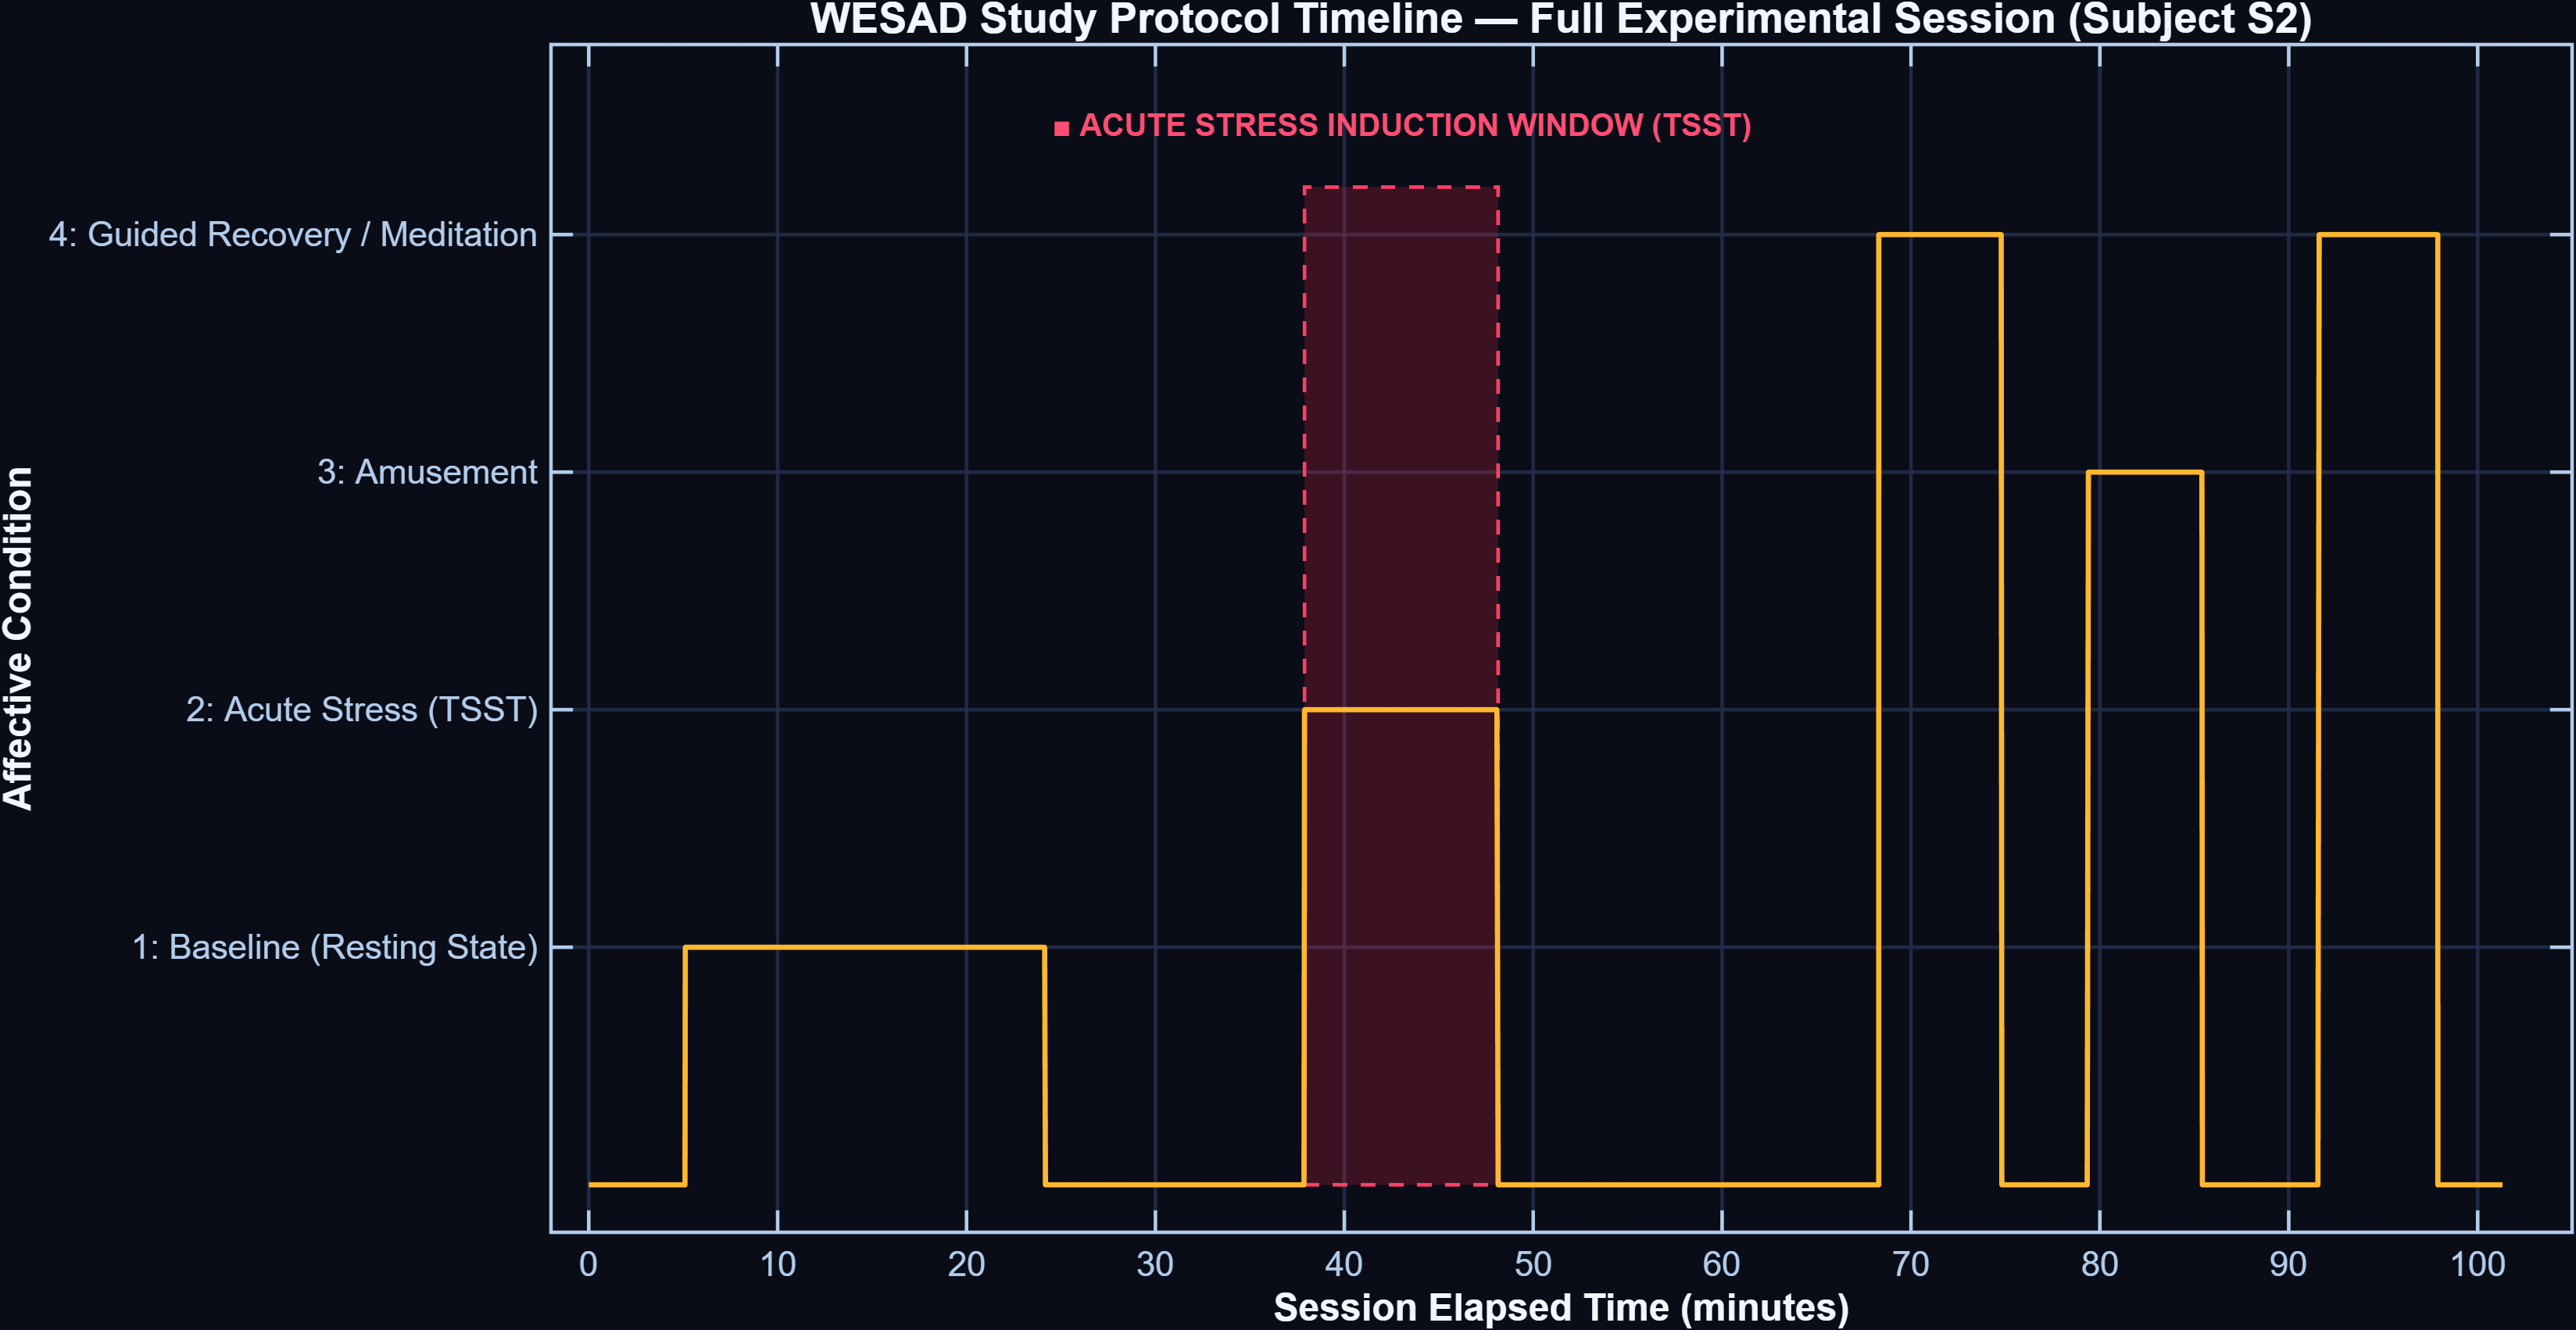
\includegraphics[width=0.98\linewidth]{figures/DEMO_Protocol_Timeline.png}
\caption{Experimental protocol timeline illustrating the temporal progression across Baseline, TSST Acute Stress, Amusement, and Meditation recovery phases.}
\label{fig:timeline}
\end{figure}

\subsection{Windowing \& Class Formulation}
Continuous ECG records were segmented into standardized 60-second sliding windows with a 50\% overlap (30-second hop). The task is formulated as binary classification: \textit{Acute Stress} ($N = 160$ valid windows) versus \textit{Non-Stress / Calm States} (Baseline + Amusement, $N = 285$ valid windows), yielding a total of 445 standardized windows across all 15 subjects.

\section{Methodology \& Signal Processing}

\subsection{Bandpass Filtering \& Adaptive R-Peak Detection}
Raw 700~Hz chest ECG signals are processed through a three-stage conditioning pipeline:
\begin{enumerate}
    \item \textbf{Zero-Phase Bandpass Filtering:} A 4th-order Butterworth bandpass filter ($0.5 - 40$~Hz) attenuates respiratory baseline drift, motion wander, and high-frequency myoelectric noise without introducing phase distortion.
    \item \textbf{MAD-Adaptive Peak Detection:} R-peaks are detected by estimating the local noise floor via the Median Absolute Deviation (MAD):
    \begin{equation}
        \text{Noise Floor} = 1.4826 \times \text{median}\left(\left|x - \text{median}(x)\right|\right)
    \end{equation}
    An adaptive prominence threshold is enforced ($\text{Prominence} \ge 3.0 \times \text{Noise Floor}$) with a refractory blanking interval of 350~ms ($\text{HR}_{\max} \le 171$~BPM).
    \item \textbf{Physiological Gating:} Inter-beat intervals $RR_i$ are recorded in seconds ($s$) and bounded by human physiological limits: $0.30\text{ s} \le RR_i \le 1.50\text{ s}$ ($300\text{--}1500\text{ ms}$, corresponding to $40\text{--}200$~BPM). Windows containing fewer than 5 valid detected beats are rejected.
\end{enumerate}

\begin{figure}[htbp]
\centering
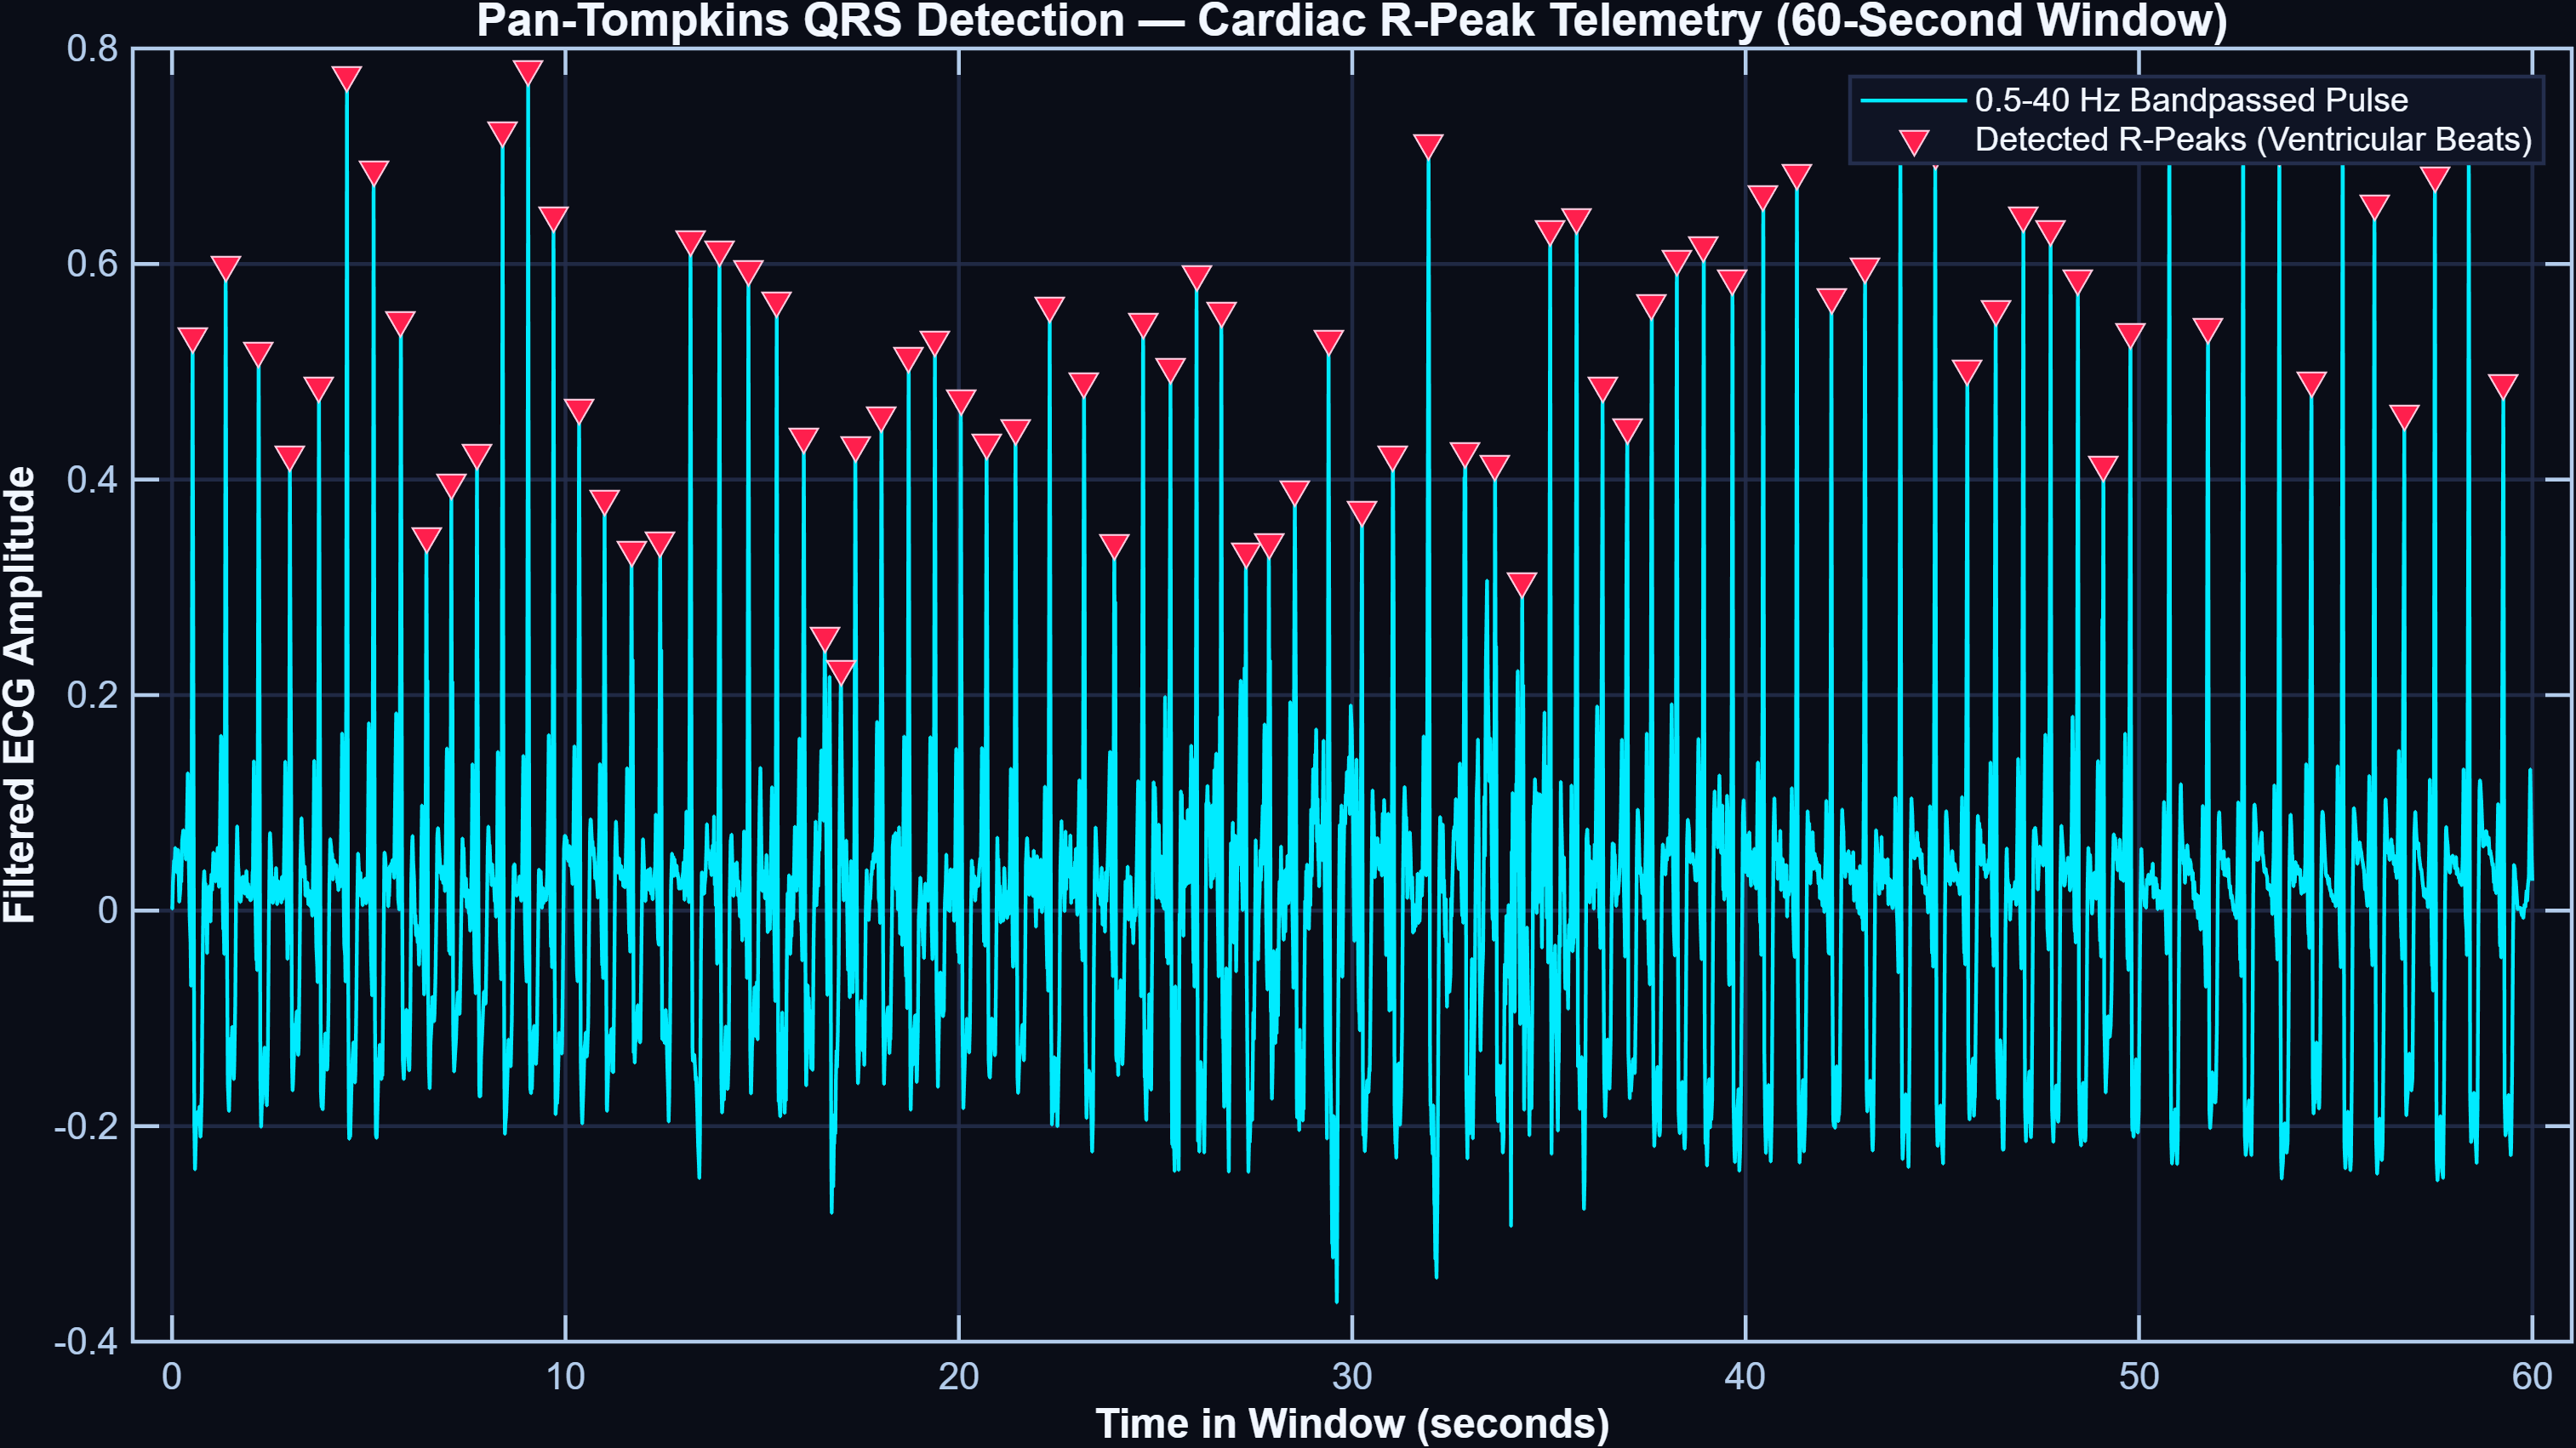
\includegraphics[width=0.98\linewidth]{figures/DEMO_Pan_Tompkins_QRS_Detection.png}
\caption{Illustrative 60-second ECG waveform conditioning demonstration: (1) Raw ECG; (2) Bandpass-filtered signal (0.5--40 Hz); (3) Squared derivative waveform; (4) Moving-window integrated signal with fiducial R-peaks (red circles). Automated multi-subject segmentation utilizes MAD-adaptive prominence detection.}
\label{fig:qrs}
\end{figure}

\subsection{Feature Engineering}
From the physiologically validated $RR$ interval sequence within each 60-second window, 13 time-domain and statistical distribution metrics are computed \cite{taskforce1996hrv, shaffer2017overview}:
MeanHR, MedianHR, StdHR, MinHR, MaxHR, MeanRR, MedianRR, SDNN, RMSSD, pNN50, RR\_CV, RR\_IQR, and HR\_IQR. Instantaneous heart rate is derived from intervals in seconds ($s$):
\begin{equation}
    \text{HR}_i = \frac{60}{RR_i} \quad (\text{BPM}, \; RR_i \text{ in seconds})
\end{equation}
In accordance with international Task Force standards \cite{taskforce1996hrv}, autonomic variability features ($\text{SDNN}$, $\text{RMSSD}$, $\text{MeanRR}$, $\text{RR}_{\text{IQR}}$) are computed on intervals scaled to milliseconds ($RR_i \times 1000$~ms):
\begin{equation}
    \text{SDNN} = \sqrt{\frac{1}{N-1} \sum_{i=1}^N \left(RR_i - \overline{RR}\right)^2} \quad (\text{ms})
\end{equation}
\begin{equation}
    \text{RMSSD} = \sqrt{\frac{1}{N-1} \sum_{i=1}^{N-1} \left(RR_{i+1} - RR_i\right)^2} \quad (\text{ms})
\end{equation}
\begin{equation}
    \text{pNN50} = \frac{\sum_{i=1}^{N-1} \mathbb{I}\left(|RR_{i+1} - RR_i| > 50\text{ ms}\right)}{N-1} \times 100\%
\end{equation}
\begin{equation}
    \text{RR\_CV} = \frac{\text{SDNN}}{\overline{RR}}
\end{equation}

For the finalized model, an optimal 8-feature representation is selected:
\begin{equation}
\begin{split}
    \mathbf{X} = [ & \text{MeanHR},\; \text{SDNN},\; \text{RMSSD},\; \text{pNN50}, \\
                   & \text{MeanRR},\; \text{RR}_{\text{CV}},\; \text{RR}_{\text{IQR}},\; \text{HR}_{\text{IQR}} ]
\end{split}
\end{equation}

\subsection{Subject-Specific Relative Normalization}
Let $X \in \mathbb{R}^D$ denote a feature vector extracted from an analysis window of subject $s$. Let $\mathcal{W}_{\text{base}}^{(s)}$ denote the collection of resting baseline windows for subject $s$. The reference baseline vector $B_s$ is defined as the empirical centroid:
\begin{equation}
    B_s = \frac{1}{|\mathcal{W}_{\text{base}}^{(s)}|} \sum_{k \in \mathcal{W}_{\text{base}}^{(s)}} X_k^{(s)}
\end{equation}
Each feature vector $X$ is then mapped to a relative fractional deviation:
\begin{equation}
    X^* = \frac{X - B_s}{|B_s| + \epsilon}
\end{equation}
where $\epsilon = 10^{-6}$ ensures numerical stability. This transformation expresses each physiological metric as a relative fractional deviation from the subject's resting baseline, centering baseline physiology around zero.

\section{Validation Protocol}
To evaluate cross-subject generalization within the WESAD cohort, all models were evaluated using \textbf{15-fold Leave-One-Subject-Out Cross-Validation with Subject-Specific Unsupervised Baseline Calibration (LOSO-CV)}:
\begin{itemize}
    \item In each fold $k \in \{1, \dots, 15\}$, the supervised model is trained strictly on the remaining 14 subjects.
    \item No stress labels or experimental task windows from test subject $k$ are ever exposed during model training.
    \item For the test subject, resting baseline windows are utilized solely to establish reference vector $B_k$ (unsupervised calibration); no stress labels from the held-out subject are ever used for model fitting.
    \item \textbf{Decision Thresholding \& Operating Points:} In the comparative multi-model benchmark (Section~\ref{subsec:ml_benchmark}), all architectures are evaluated at the standard decision threshold of $\tau = 0.50$, where Logistic Regression achieves 92.13\% accuracy and 88.29\% F1-score without threshold adjustment. To examine operational trade-offs under class imbalance (stress prevalence: 36.0\%), decision thresholds from $\tau = 0.10$ to $0.90$ (step 0.01) were systematically evaluated during calibration, and an operating cutoff of $\tau = 0.35$ was selected to prioritize stress recall while preserving high balanced accuracy ($>$91\%). Crucially, the primary discrimination metrics, ROC-AUC (0.9494) and PR-AUC (0.9467), evaluate model performance across the entire continuum of operating thresholds independently of any specific cutoff.
\end{itemize}

\section{Experimental Results}

\subsection{Primary Benchmark Performance}
Evaluated across all 445 standardized windows from all 15 subjects under 15-fold LOSO-CV, the proposed classifier achieves the validated scorecard summarized in Table~\ref{tab:scorecard}.

\begin{table}[htbp]
\caption{Validated 15-Fold LOSO Primary Performance Scorecard (calibrated operating point $\tau = 0.35$)}
\label{tab:scorecard}
\centering
\resizebox{\columnwidth}{!}{%
\begin{tabular}{lcp{3.4cm}}
\toprule
\textbf{Metric} & \textbf{Result} & \textbf{Operational Interpretation} \\
\midrule
Accuracy & \textbf{92.36\%} & 411 / 445 total windows correct \\
Sensitivity (Recall) & \textbf{86.25\%} & 138 / 160 stress windows detected \\
Specificity & \textbf{95.79\%} & 273 / 285 non-stress windows correct \\
Precision & \textbf{92.00\%} & 138 / 150 stress predictions correct \\
F1-Score & \textbf{89.03\%} & Harmonic mean of recall \& precision \\
Balanced Accuracy & \textbf{91.02\%} & Unbiased average across classes \\
ROC-AUC & \textbf{0.9494} & Area under ROC curve \\
PR-AUC & \textbf{0.9467} & Precision-Recall trajectory area \\
Confusion Matrix & \multicolumn{2}{l}{TN: 273, FP: 12, FN: 22, TP: 138} \\
\bottomrule
\end{tabular}%
}
\end{table}

\begin{figure}[htbp]
\centering
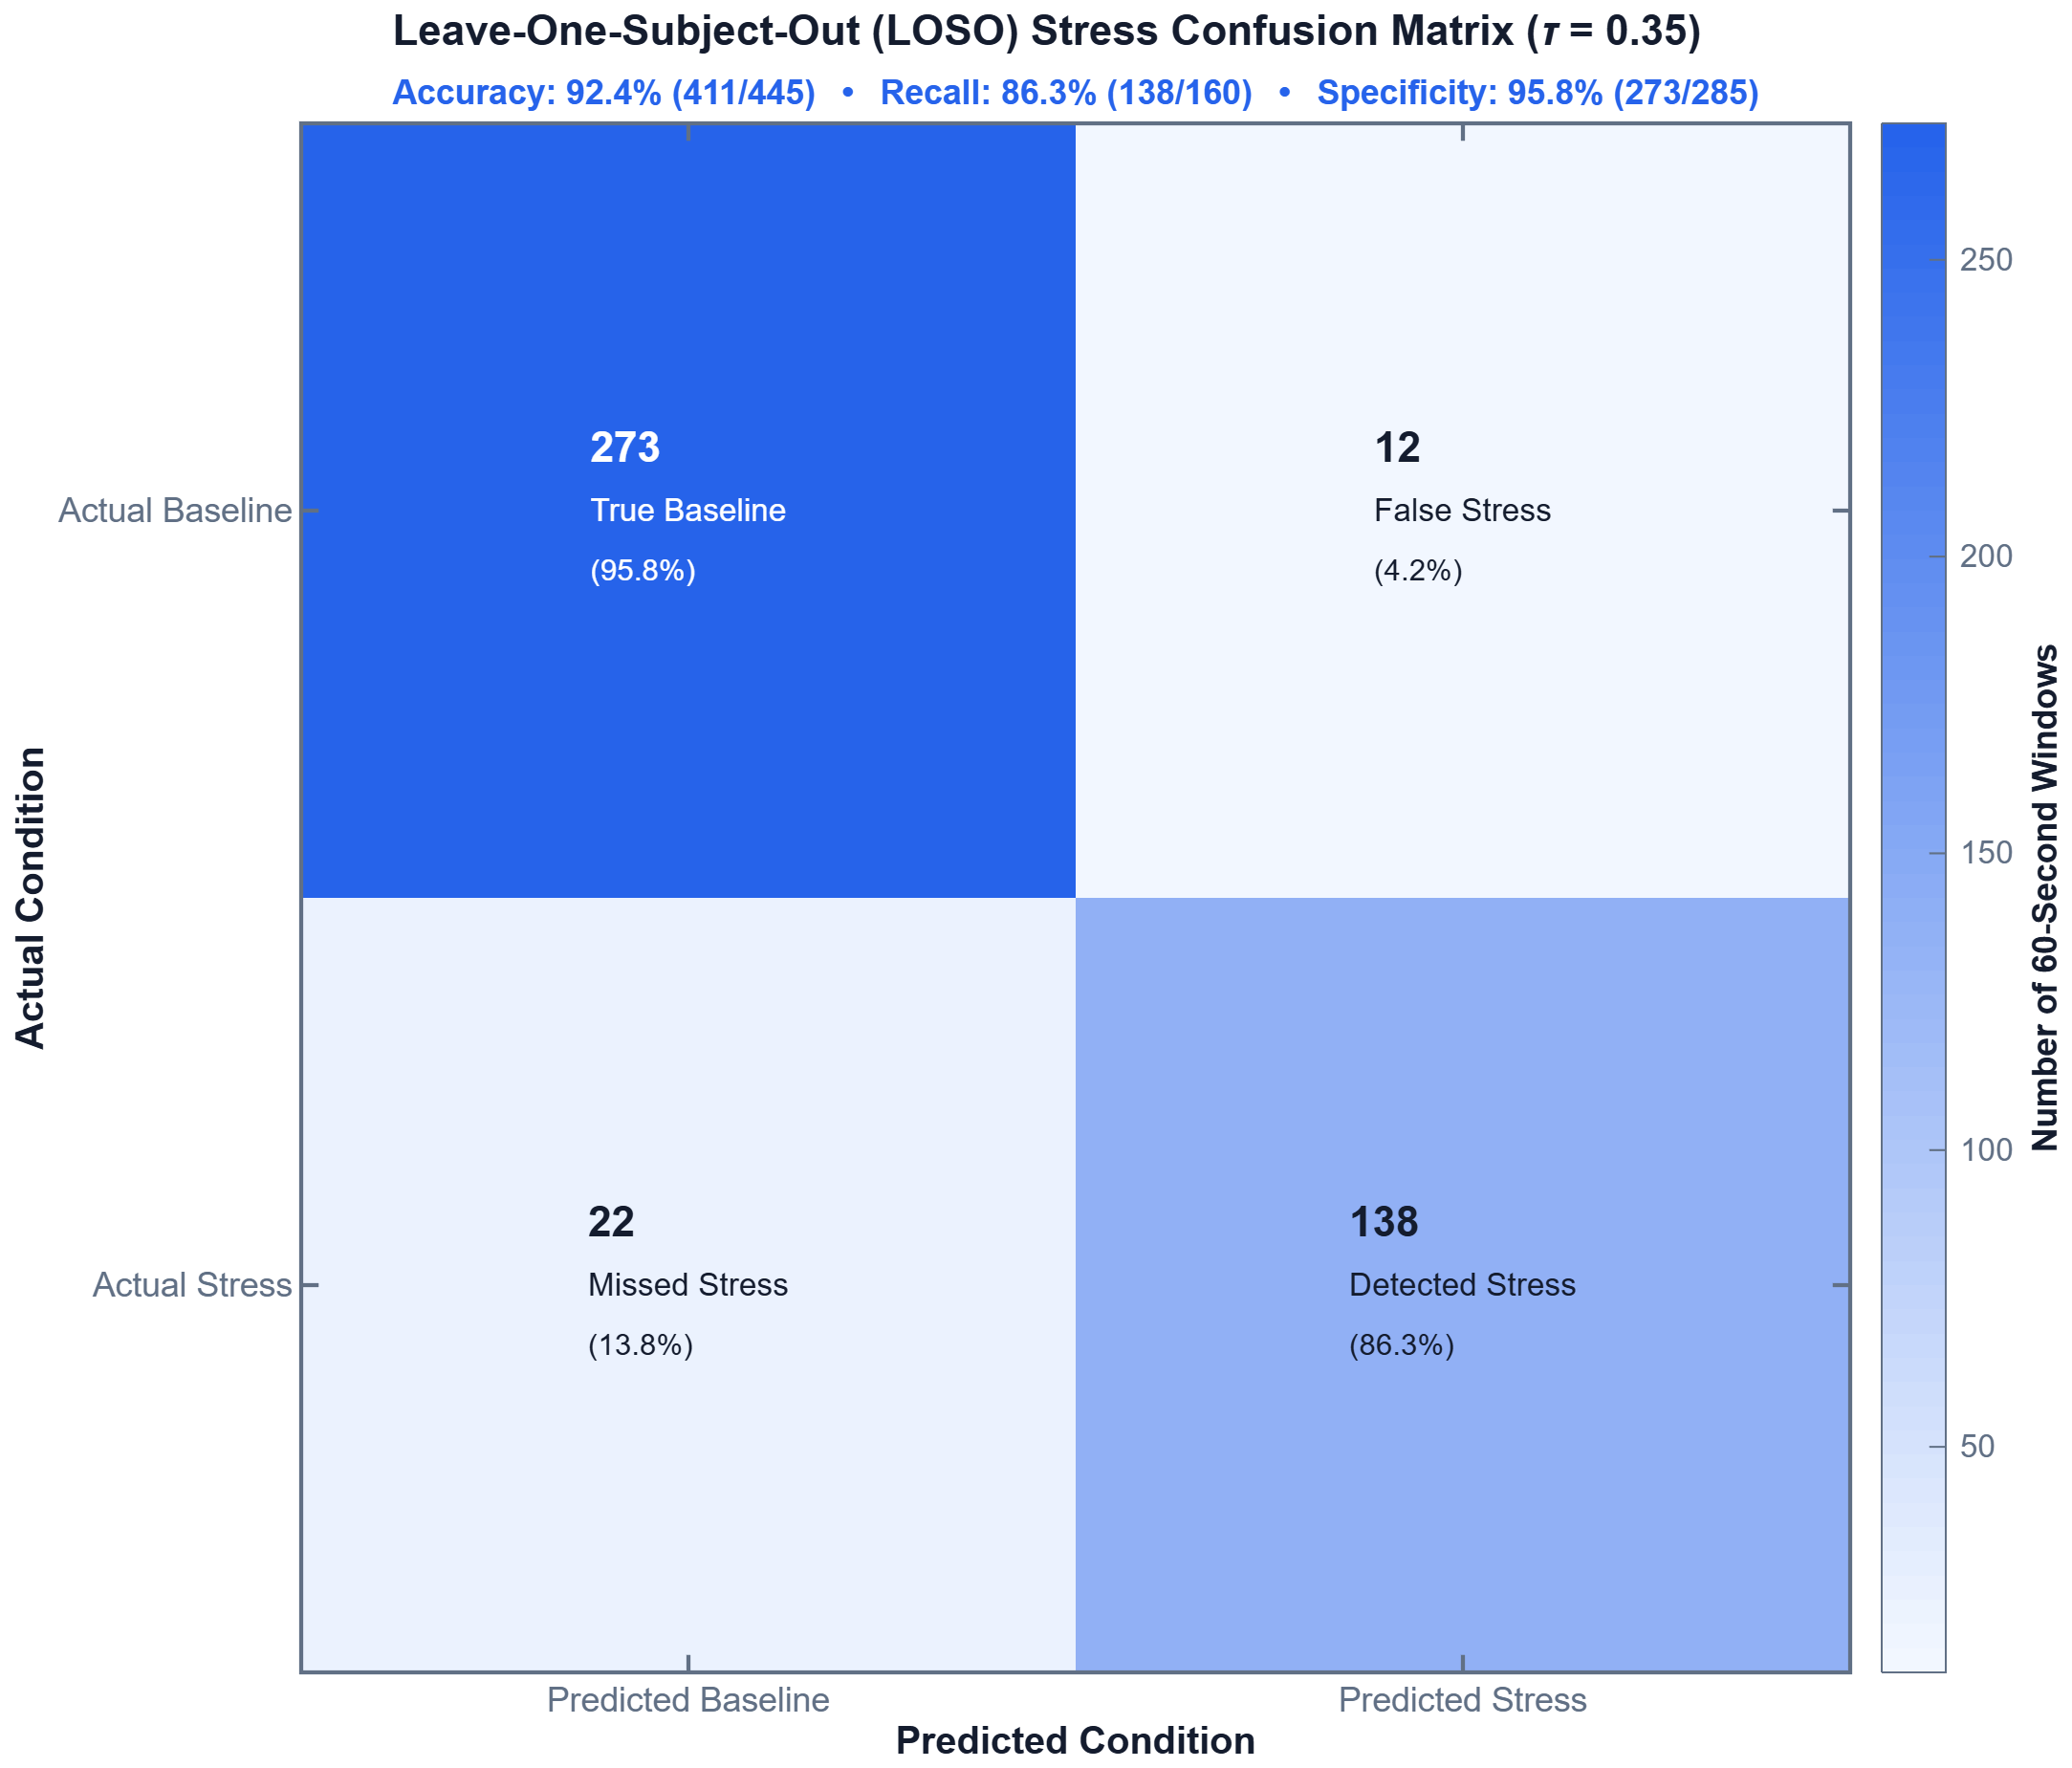
\includegraphics[width=0.88\linewidth]{figures/FINAL_Confusion_Matrix.png}
\caption{15-Fold LOSO confusion matrix showing 273/285 non-stress windows (95.8\%) and 138/160 stress windows (86.3\%) correctly classified.}
\label{fig:cm}
\end{figure}

\begin{figure}[htbp]
\centering
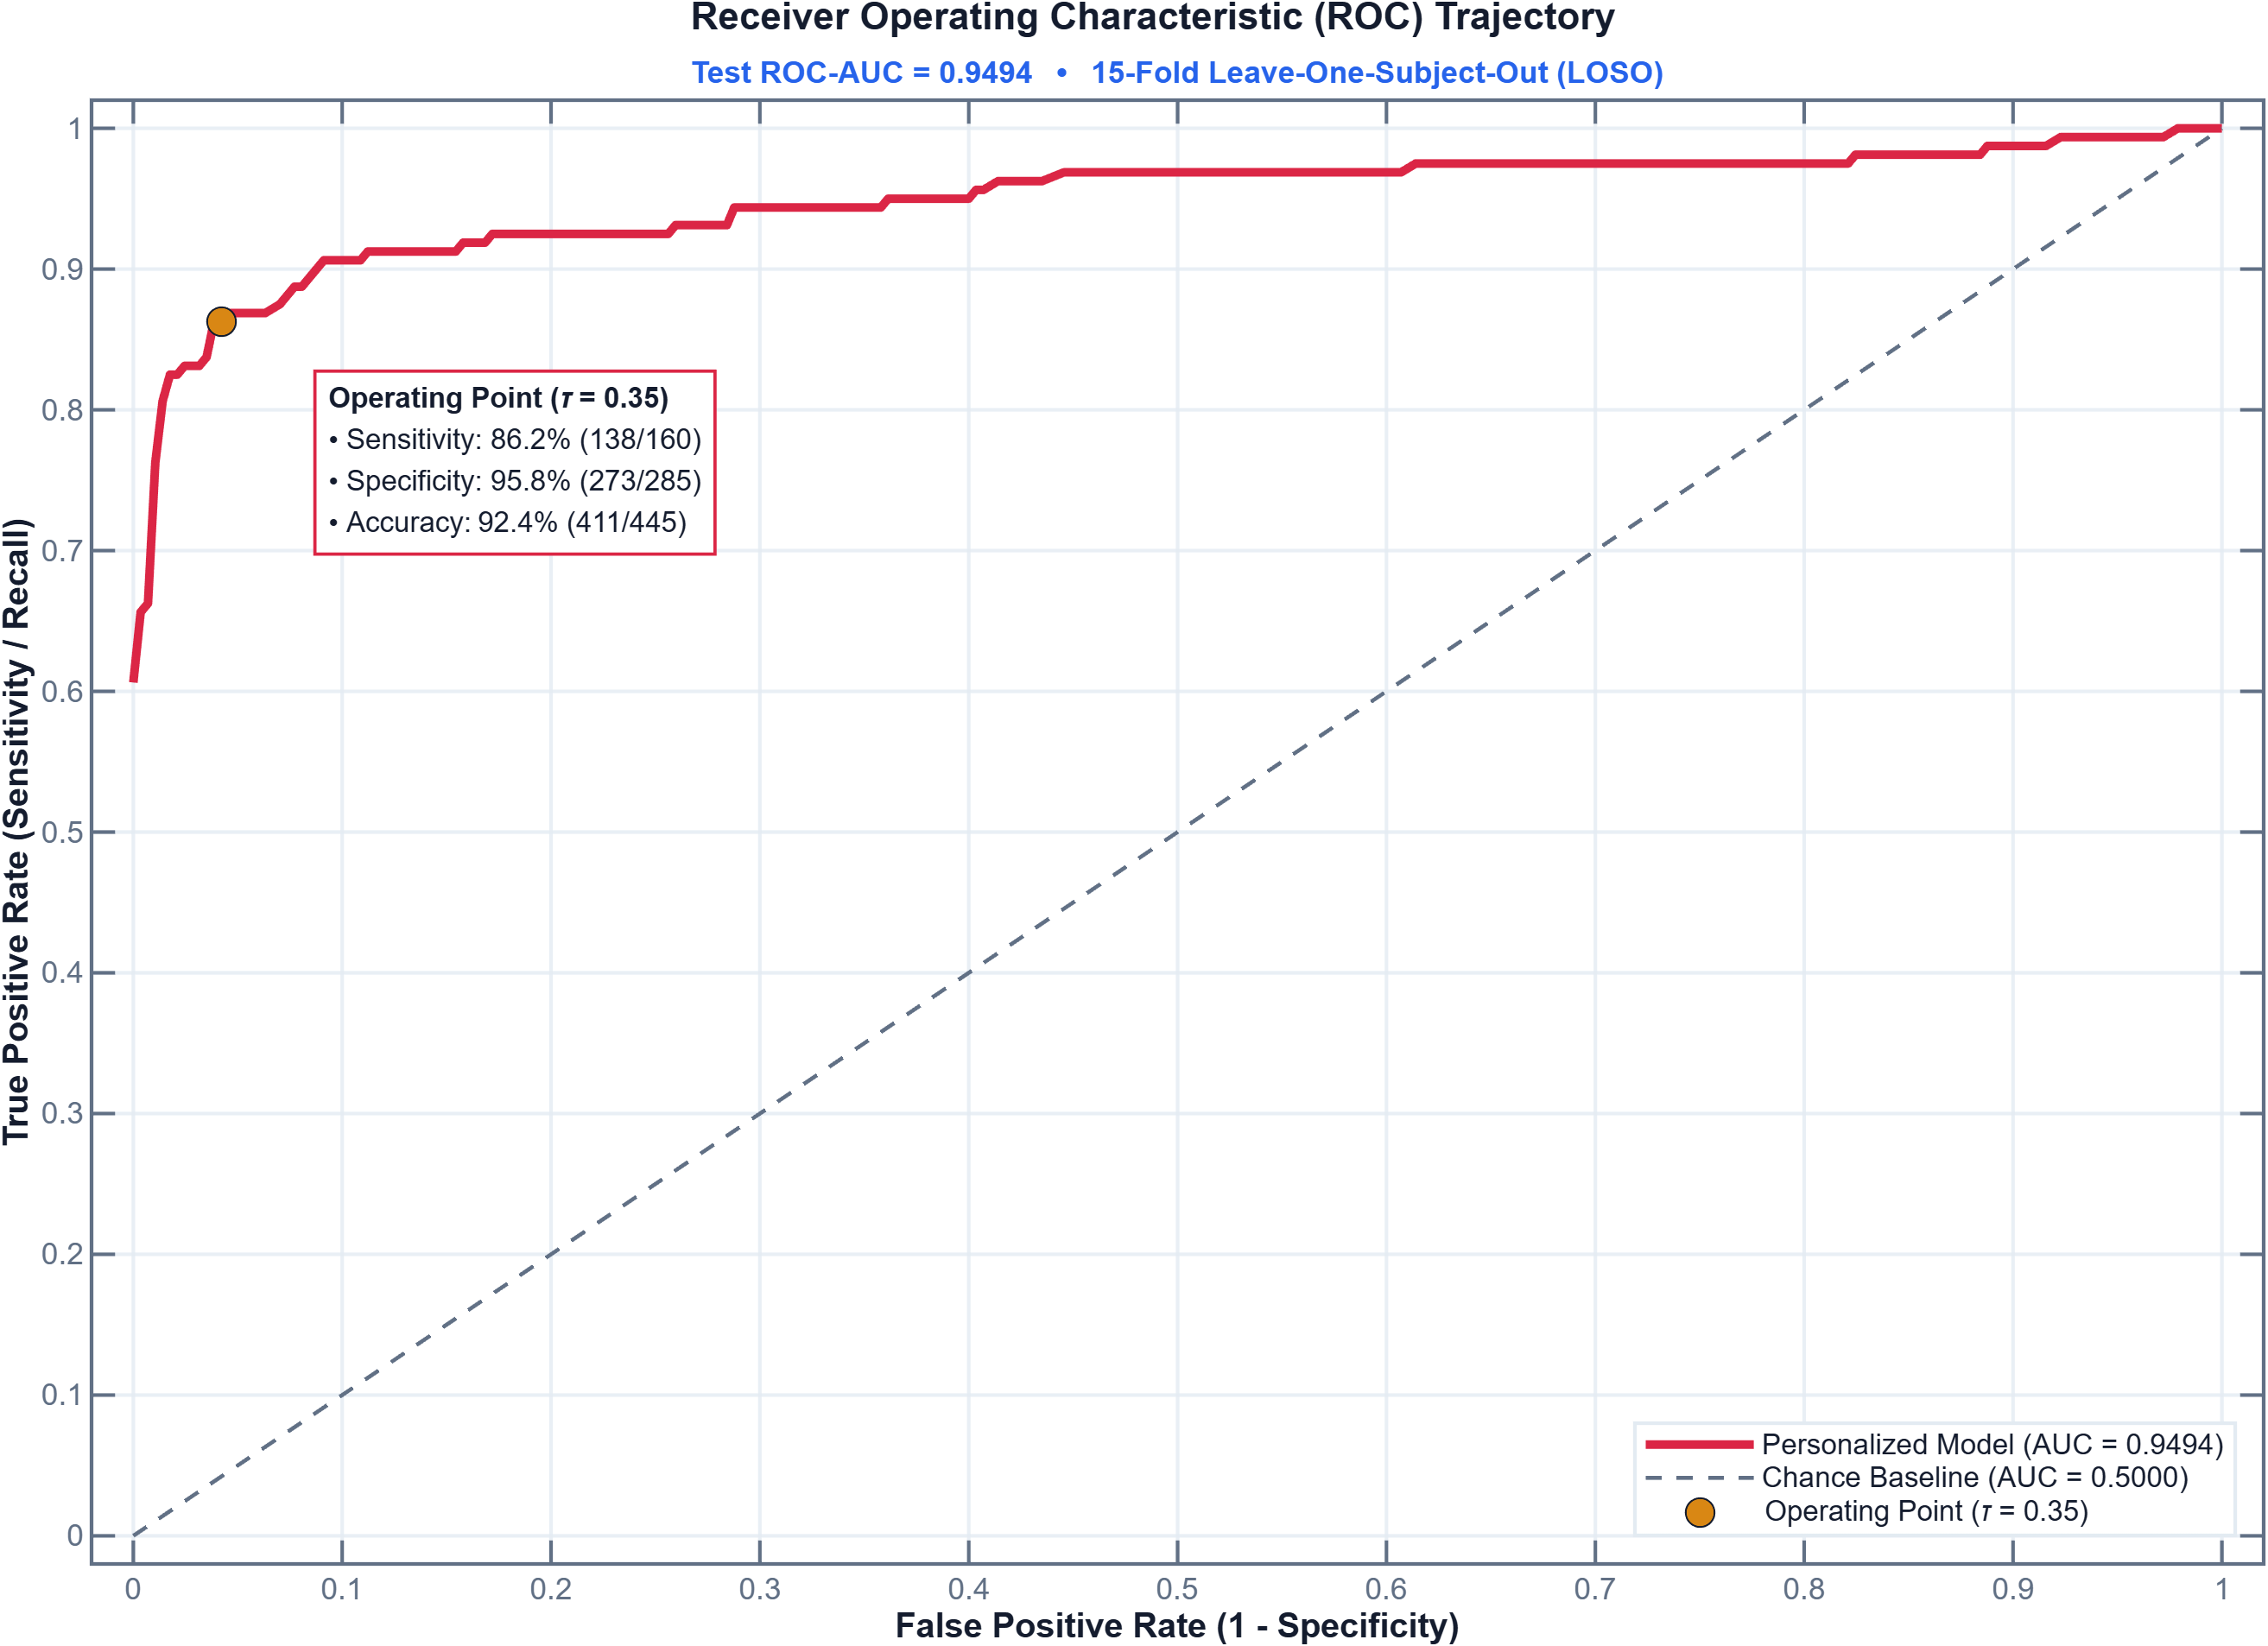
\includegraphics[width=0.88\linewidth]{figures/FINAL_ROC_Curve.png}
\caption{Cross-validated ROC curve (AUC = 0.9494) with the operating threshold ($\tau = 0.35$) highlighted.}
\label{fig:roc}
\end{figure}

\subsection{Comparison with Published WESAD Benchmark}
Table~\ref{tab:lit_comparison} compares the proposed method against the published WESAD benchmark by Schmidt \textit{et al.} \cite{schmidt2018wesad}. Compared with the cited published chest-ECG results reported under 15-fold LOSO evaluation, applying subject-specific relative normalization exceeds the published uncalibrated baselines by \textbf{+8.5\% to +13.3\% in accuracy} and \textbf{+13.9\% to +17.6\% in F1-score}.

\begin{table}[htbp]
\caption{Comparison with Published WESAD Benchmark \cite{schmidt2018wesad}}
\label{tab:lit_comparison}
\centering
\resizebox{\columnwidth}{!}{%
\begin{tabular}{llcc}
\toprule
\textbf{Study / Model} & \textbf{Normalization} & \textbf{Accuracy} & \textbf{F1-Score} \\
\midrule
Schmidt \textit{et al.} (Decision Tree) & None (Global) & 79.03\% & 71.43\% \\
Schmidt \textit{et al.} (Random Forest) & None (Global) & 83.84\% & 75.12\% \\
This Study (Uncalibrated Baseline) & None (Global) & 81.57\% & 73.03\% \\
\textbf{This Study (Personalized Classifier)} & \textbf{Relative ($X^*$)} & \textbf{92.36\%} & \textbf{89.03\%} \\
\bottomrule
\end{tabular}%
}
\end{table}

\subsection{Cross-Architecture Machine Learning Benchmark}
\label{subsec:ml_benchmark}
To determine whether the gains of relative normalization generalize across different model classes, we evaluated six machine learning architectures under identical 15-fold LOSO cross-validation (Table~\ref{tab:ml_benchmark}). All architectures achieve ROC-AUC $\ge 0.937$, indicating strong linear and nonlinear separability across diverse model classes. All comparative benchmark metrics in Table~\ref{tab:ml_benchmark} are evaluated at the default threshold $\tau = 0.50$, whereas Table~\ref{tab:scorecard} reflects the sensitivity-focused operating point at $\tau = 0.35$. The primary MATLAB Logistic Regression classifier and the Python cross-architecture benchmark represent separate implementations; minor differences in solver regularization and numerical optimization account for the small variation in ROC-AUC (0.9494 vs. 0.9493).

\begin{table}[htbp]
\caption{Multi-Model 15-Fold LOSO Benchmark Comparison (evaluated at default threshold $\tau = 0.50$; the calibrated model in Table~\ref{tab:scorecard} operates at $\tau = 0.35$)}
\label{tab:ml_benchmark}
\centering
\resizebox{\columnwidth}{!}{%
\begin{tabular}{lcccc}
\toprule
\textbf{Architecture} & \textbf{Acc (\%)} & \textbf{F1 (\%)} & \textbf{ROC-AUC} & \textbf{PR-AUC} \\
\midrule
\textbf{Logistic Regression (L2)} & \textbf{92.13} & \textbf{88.29} & \textbf{0.9493} & \textbf{0.9467} \\
Multilayer Perceptron (MLP) & 91.69 & 87.87 & 0.9375 & 0.9327 \\
Support Vector Machine (RBF) & 91.46 & 87.42 & 0.9524 & 0.9441 \\
Random Forest (100 Trees) & 90.34 & 85.90 & 0.9426 & 0.9301 \\
Extra Trees Classifier & 89.89 & 84.43 & 0.9494 & 0.9391 \\
HistGradientBoosting & 89.21 & 84.31 & 0.9459 & 0.9375 \\
\bottomrule
\end{tabular}%
}
\end{table}

\begin{figure}[htbp]
\centering
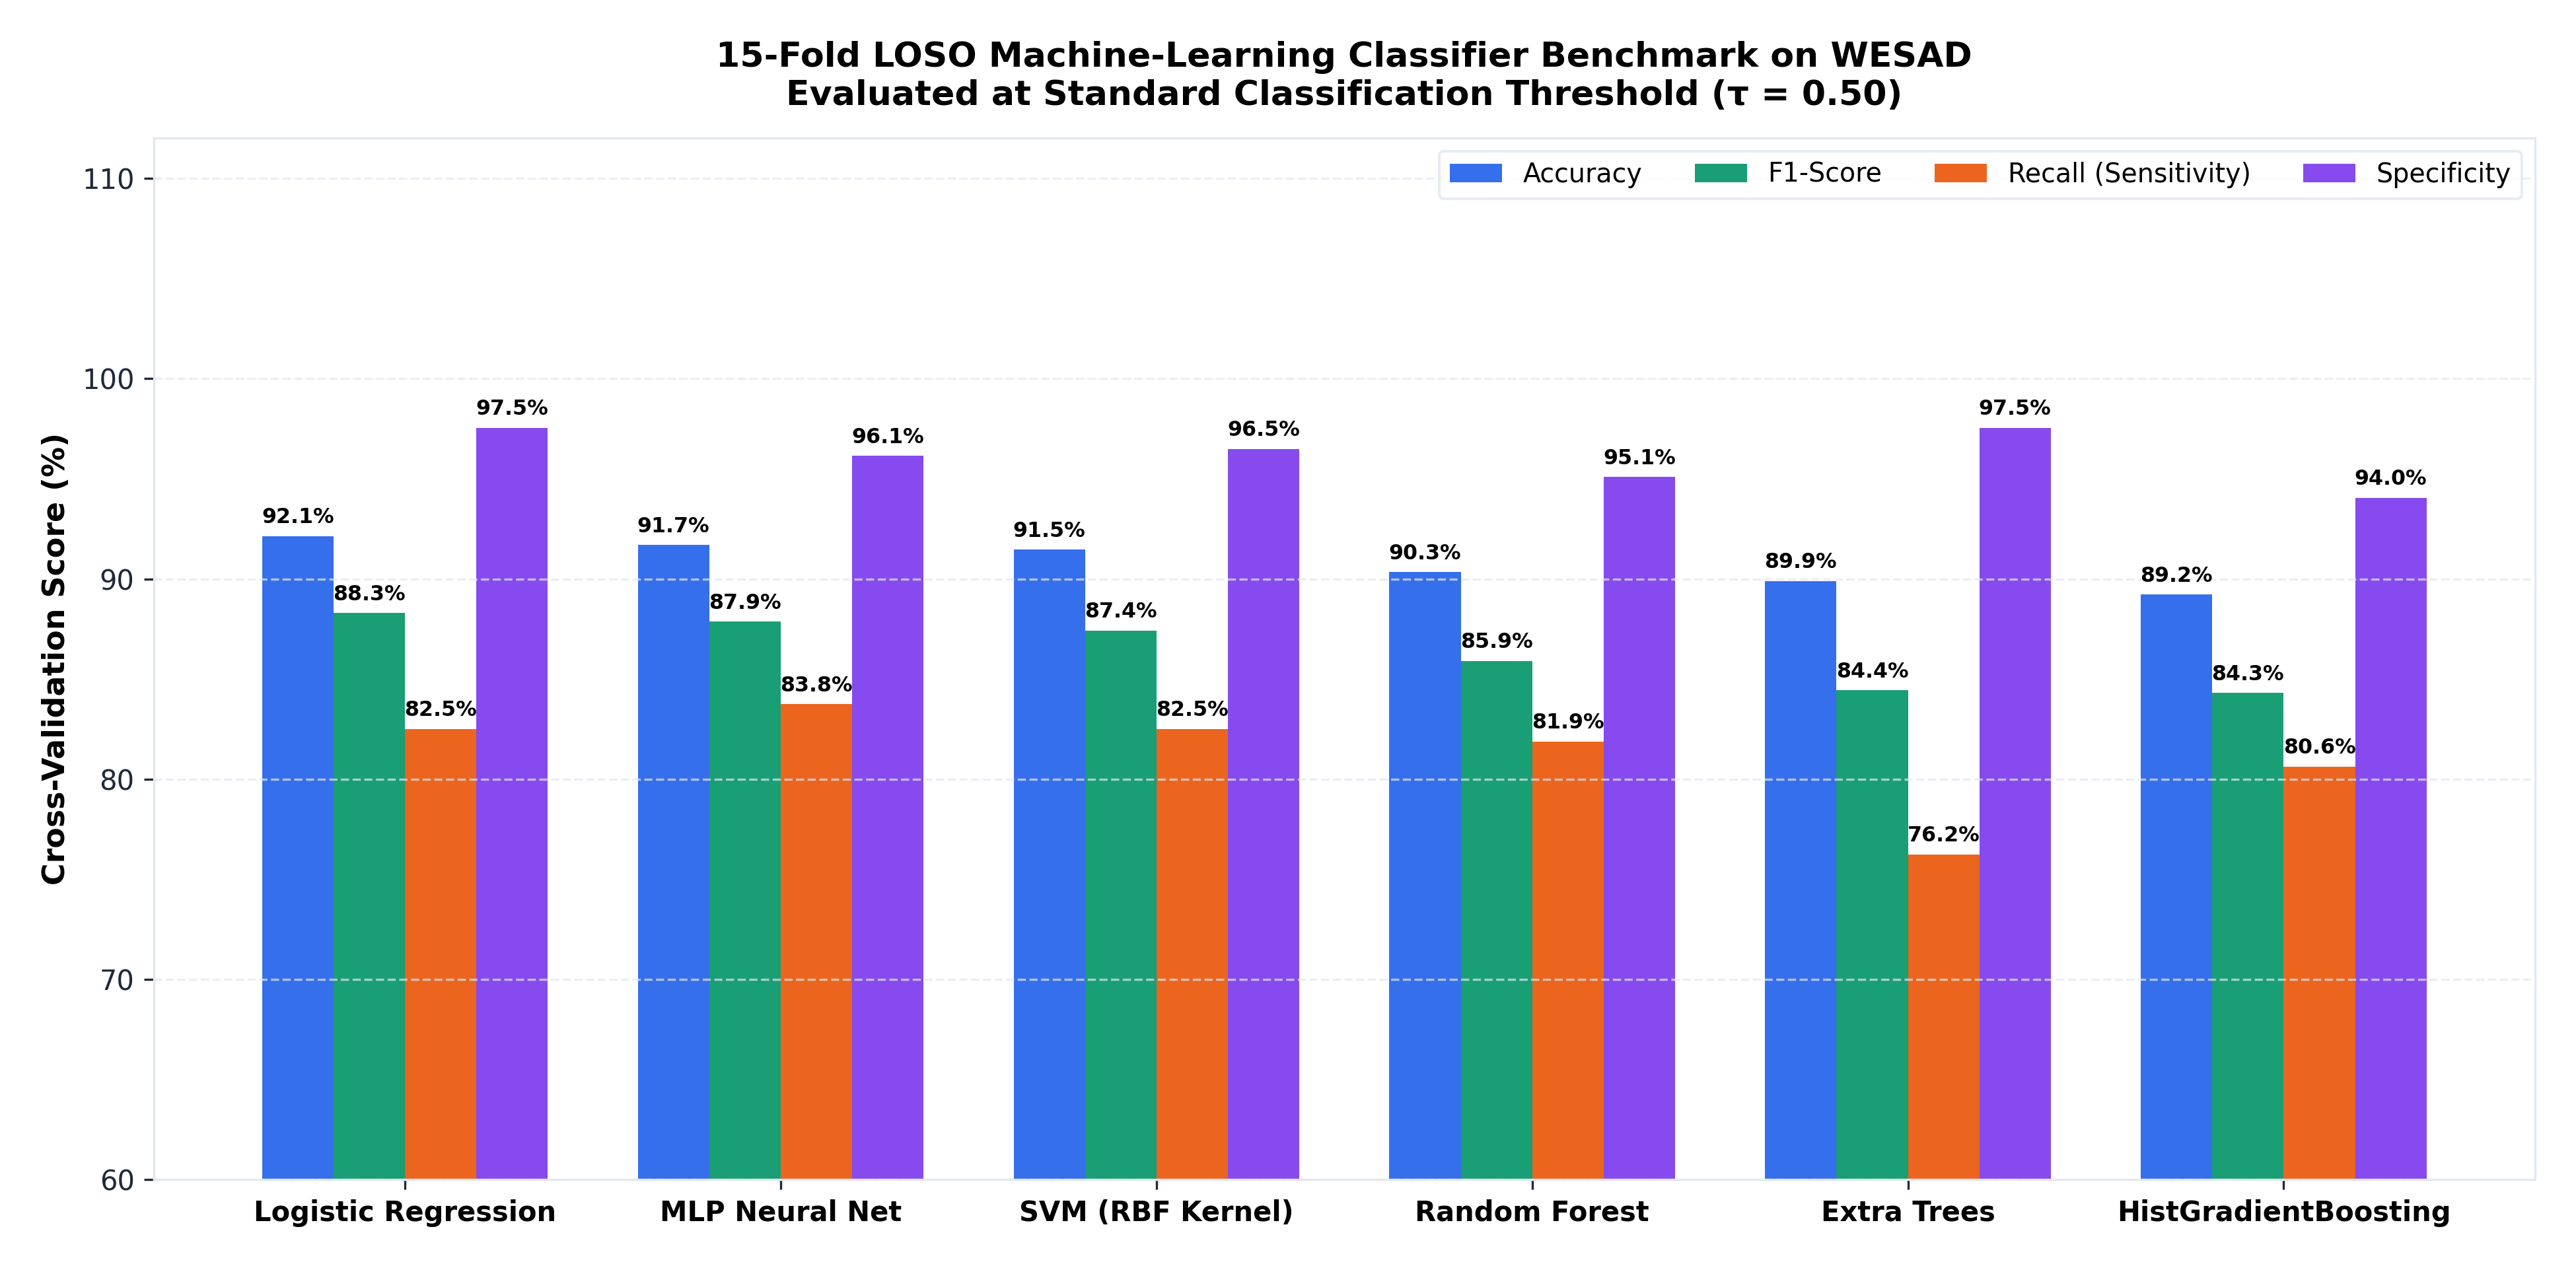
\includegraphics[width=0.98\linewidth]{figures/ML_Model_Benchmark_Bars.png}
\caption{Performance metrics across six machine learning architectures under 15-fold LOSO cross-validation on held-out test subjects.}
\label{fig:bars}
\end{figure}

\subsection{Ablation Study: Feature Expansion vs. Normalization}
To isolate the contribution of feature expansion versus baseline normalization, we evaluated four progressive configurations under identical 15-fold LOSO conditions (Table~\ref{tab:ablation}). While expanding the feature set from 1 to 13 raw metrics provides modest gains (+4.49\% Acc, +8.69\% F1), applying baseline calibration yields a substantial leap of \textbf{+10.79\% in accuracy and +16.00\% in F1-score}.

\begin{table}[htbp]
\caption{Four-Stage Model Progression \& Feature Ablation}
\label{tab:ablation}
\centering
\resizebox{\columnwidth}{!}{%
\begin{tabular}{llccc}
\toprule
\textbf{ID} & \textbf{Configuration} & \textbf{Acc (\%)} & \textbf{F1 (\%)} & \textbf{Recall (\%)} \\
\midrule
M1 & Raw MeanHR (Uncalibrated) & 77.08 & 64.34 & 61.25 \\
M2 & 4 Time-Domain (Uncalibrated) & 80.90 & 70.59 & 67.50 \\
M3 & 13 Metrics (Uncalibrated) & 81.57 & 73.03 & 68.75 \\
\textbf{M4} & \textbf{Personalized ($X^*$ Calibrated)} & \textbf{92.36} & \textbf{89.03} & \textbf{86.25} \\
\bottomrule
\end{tabular}%
}
\end{table}

\begin{figure}[htbp]
\centering
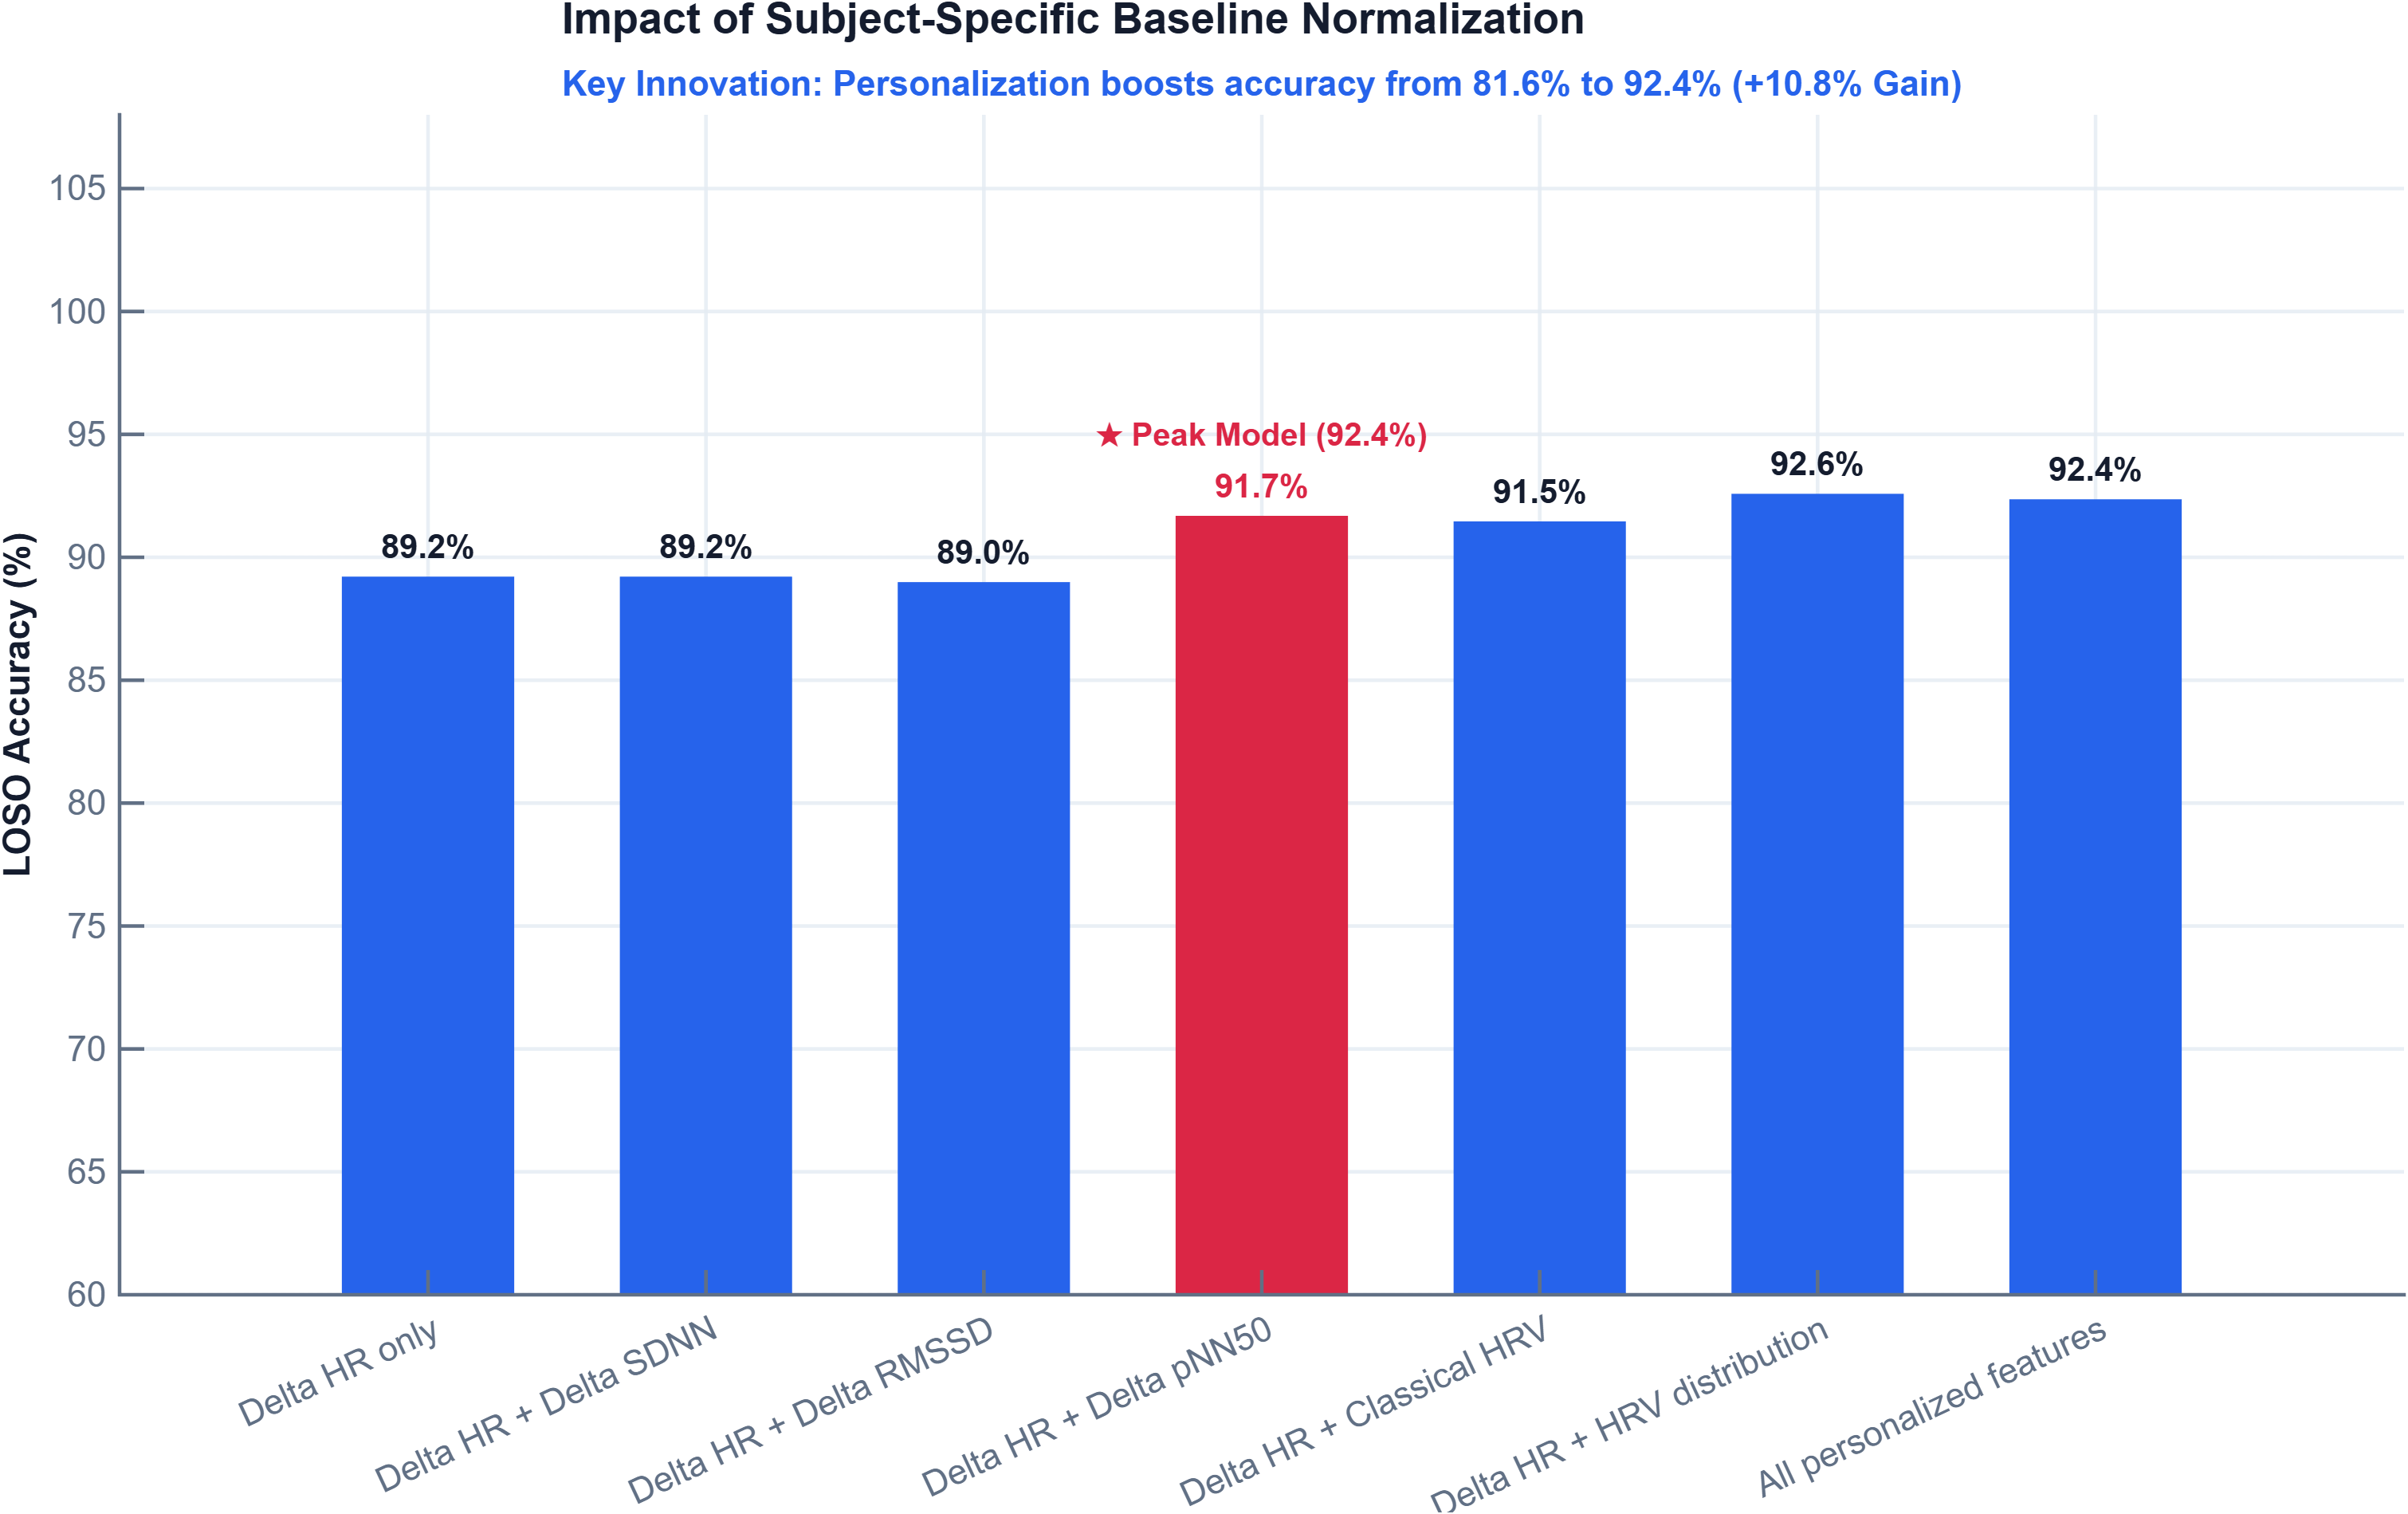
\includegraphics[width=0.95\linewidth]{figures/FINAL_Personalized_Feature_Ablation.png}
\caption{Four-stage model progression demonstrating that baseline calibration provides the primary performance leap (+10.79\% Acc, +16.00\% F1).}
\label{fig:ablation}
\end{figure}

\subsection{Feature Importance \& Physiological Attribution}
We evaluated feature importance via 30 independent random permutations per feature across each of the 15 test folds ($15 \times 30 = 450$ trials per feature) for both Logistic Regression and Random Forest models, paired with standardized logistic regression odds ratios ($e^{w_i}$ derived following z-score standardization of baseline-relative features):
\begin{itemize}
    \item \textbf{Cardiac Interval Compression ($\Delta\text{MeanRR}$):} Exhibited the largest discriminative degradation upon shuffling ($\Delta\text{AUC} = 0.1766$, $\Delta\text{F1} = 0.2321$, Odds Ratio = 0.0645), confirming that RR interval shortening is the primary statistical indicator of acute stress.
    \item \textbf{Heart Rate Elevation ($\Delta\text{MeanHR}$):} Strongly increases stress odds (Odds Ratio = 5.6453, $\Delta\text{AUC} = 0.0203$, $\Delta\text{F1} = 0.1021$ in LR and $0.1401$ in Random Forest), consistent with sympathetic chronotropic acceleration during TSST cognitive challenge.
    \item \textbf{Interval Dispersion ($\Delta\text{pNN50}$):} Demonstrates substantial predictive weight (Odds Ratio = 4.0784, $\Delta\text{AUC} = 0.0596$, $\Delta\text{F1} = 0.0606$), consistent with rapid autonomic vagal modulation shifts during cognitive challenge.
    \item \textbf{Autonomic Variability ($\Delta\text{SDNN}$):} Sustained total variability acts as a protective calm indicator (Odds Ratio = 0.4625, $\Delta\text{AUC} = 0.0078$, $\Delta\text{F1} = 0.0042$), where an Odds Ratio $< 1.0$ is physiologically compatible with preserved autonomic variability during homeostatic resting calm.
\end{itemize}

\begin{figure}[htbp]
\centering
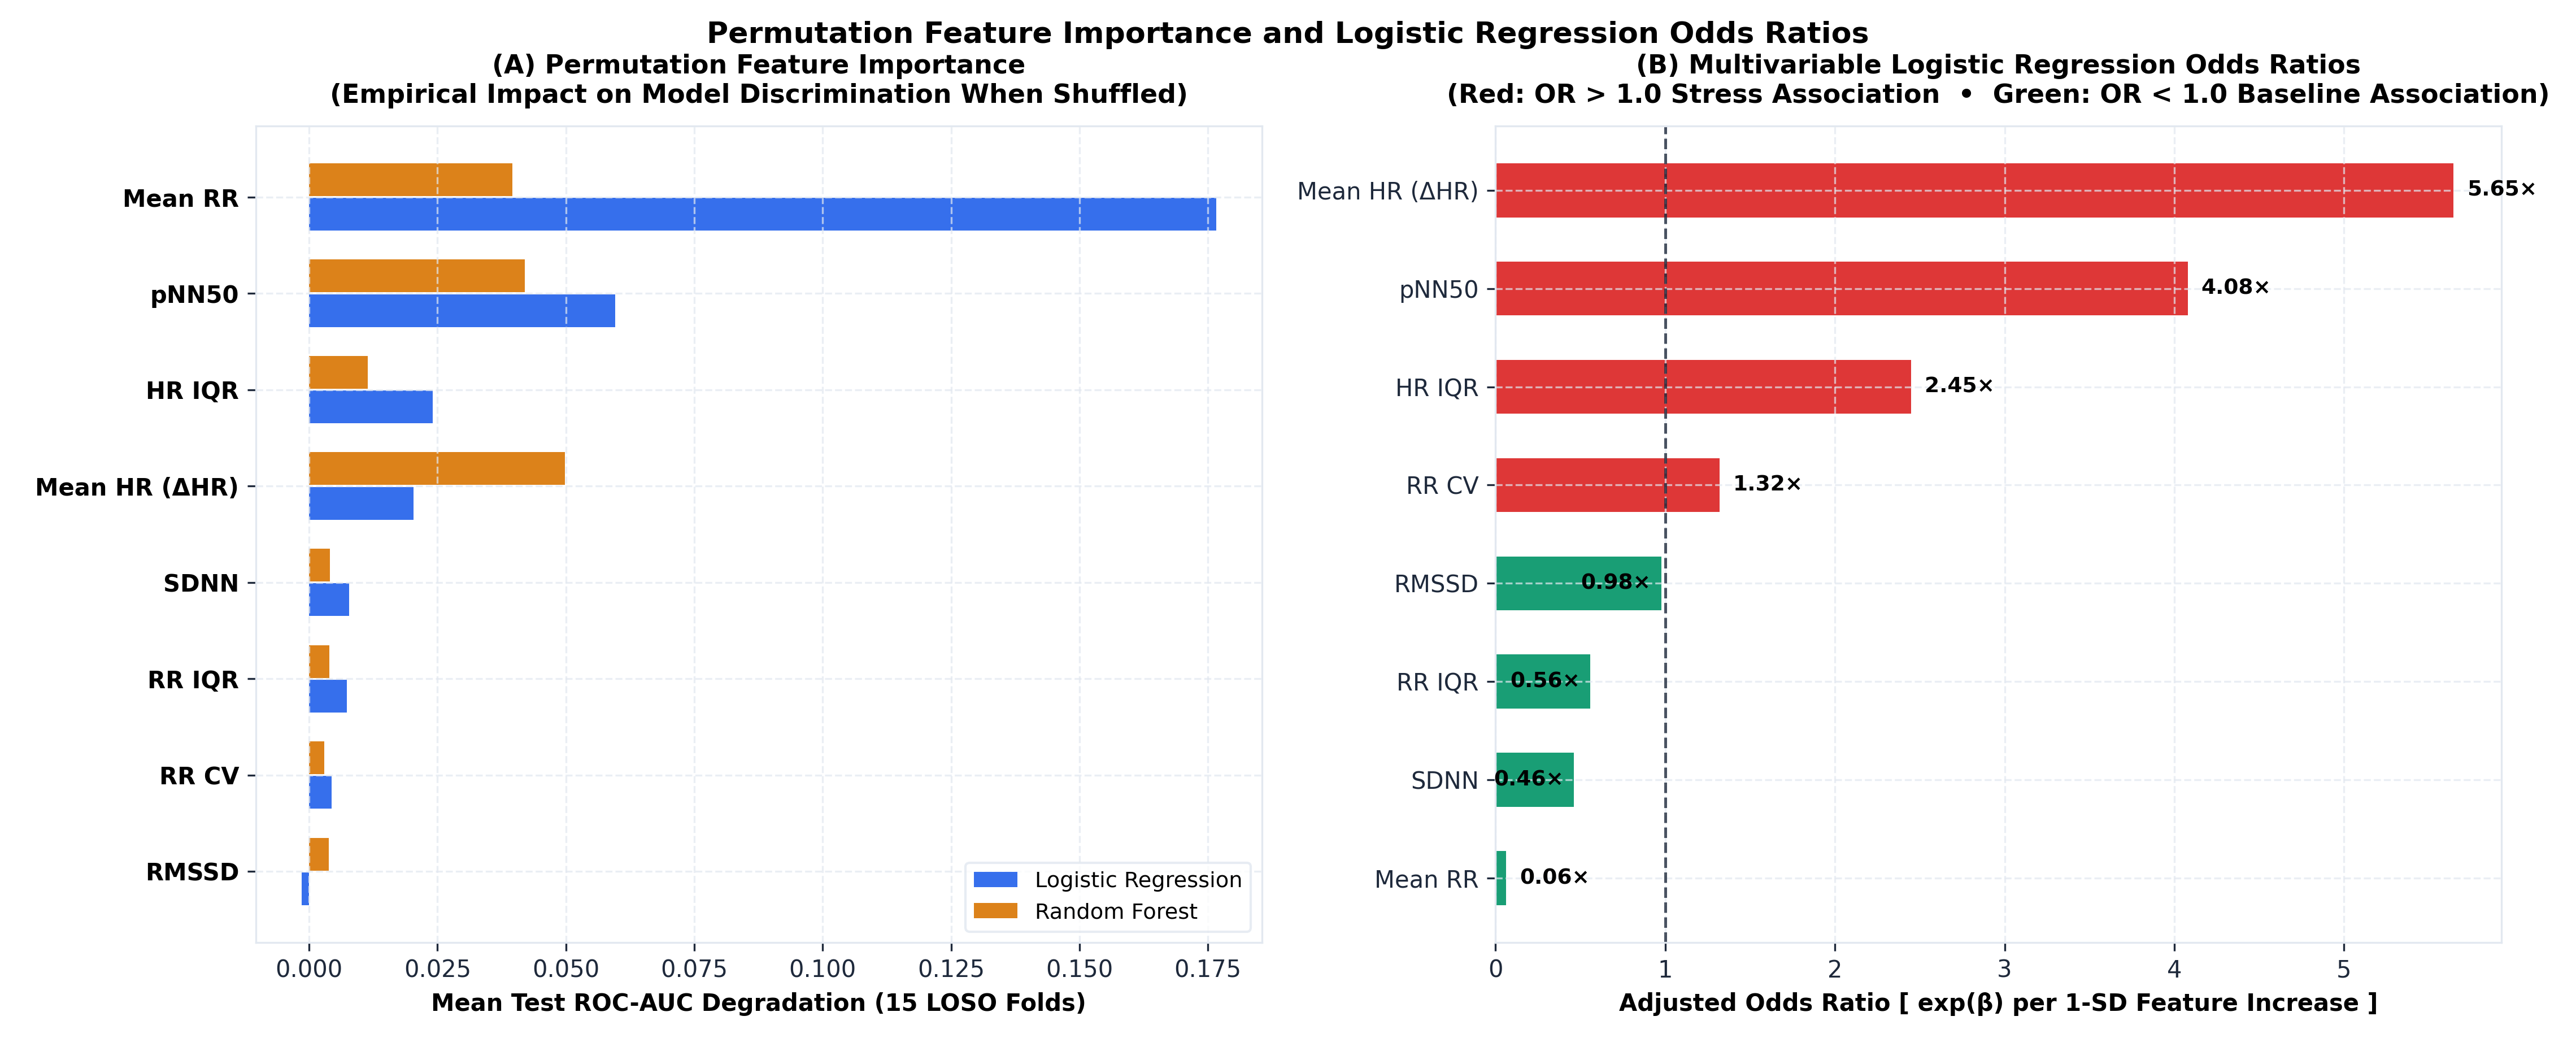
\includegraphics[width=0.98\linewidth]{figures/ML_Feature_Importance_Permutation.png}
\caption{(Left) Test ROC-AUC drop under 30-repeat permutation across 15 LOSO folds; (Right) Standardized odds ratios indicating the magnitude and direction of feature weights.}
\label{fig:importance}
\end{figure}

\subsection{Subject Heterogeneity \& Low-Reactivity Discussion}
Subject-specific stress detection rates across all 15 subjects (Figure~\ref{fig:subjects}) demonstrate robust cross-subject generalization: 14 of 15 subjects exhibit successful acute stress detection ($>0\%$ sensitivity, capturing 138 of 160 total stress windows, 86.25\%), with 13 of 15 achieving $\ge 75.0\%$ recall and 9 of 15 achieving complete $100.0\%$ recall.

\begin{figure}[htbp]
\centering
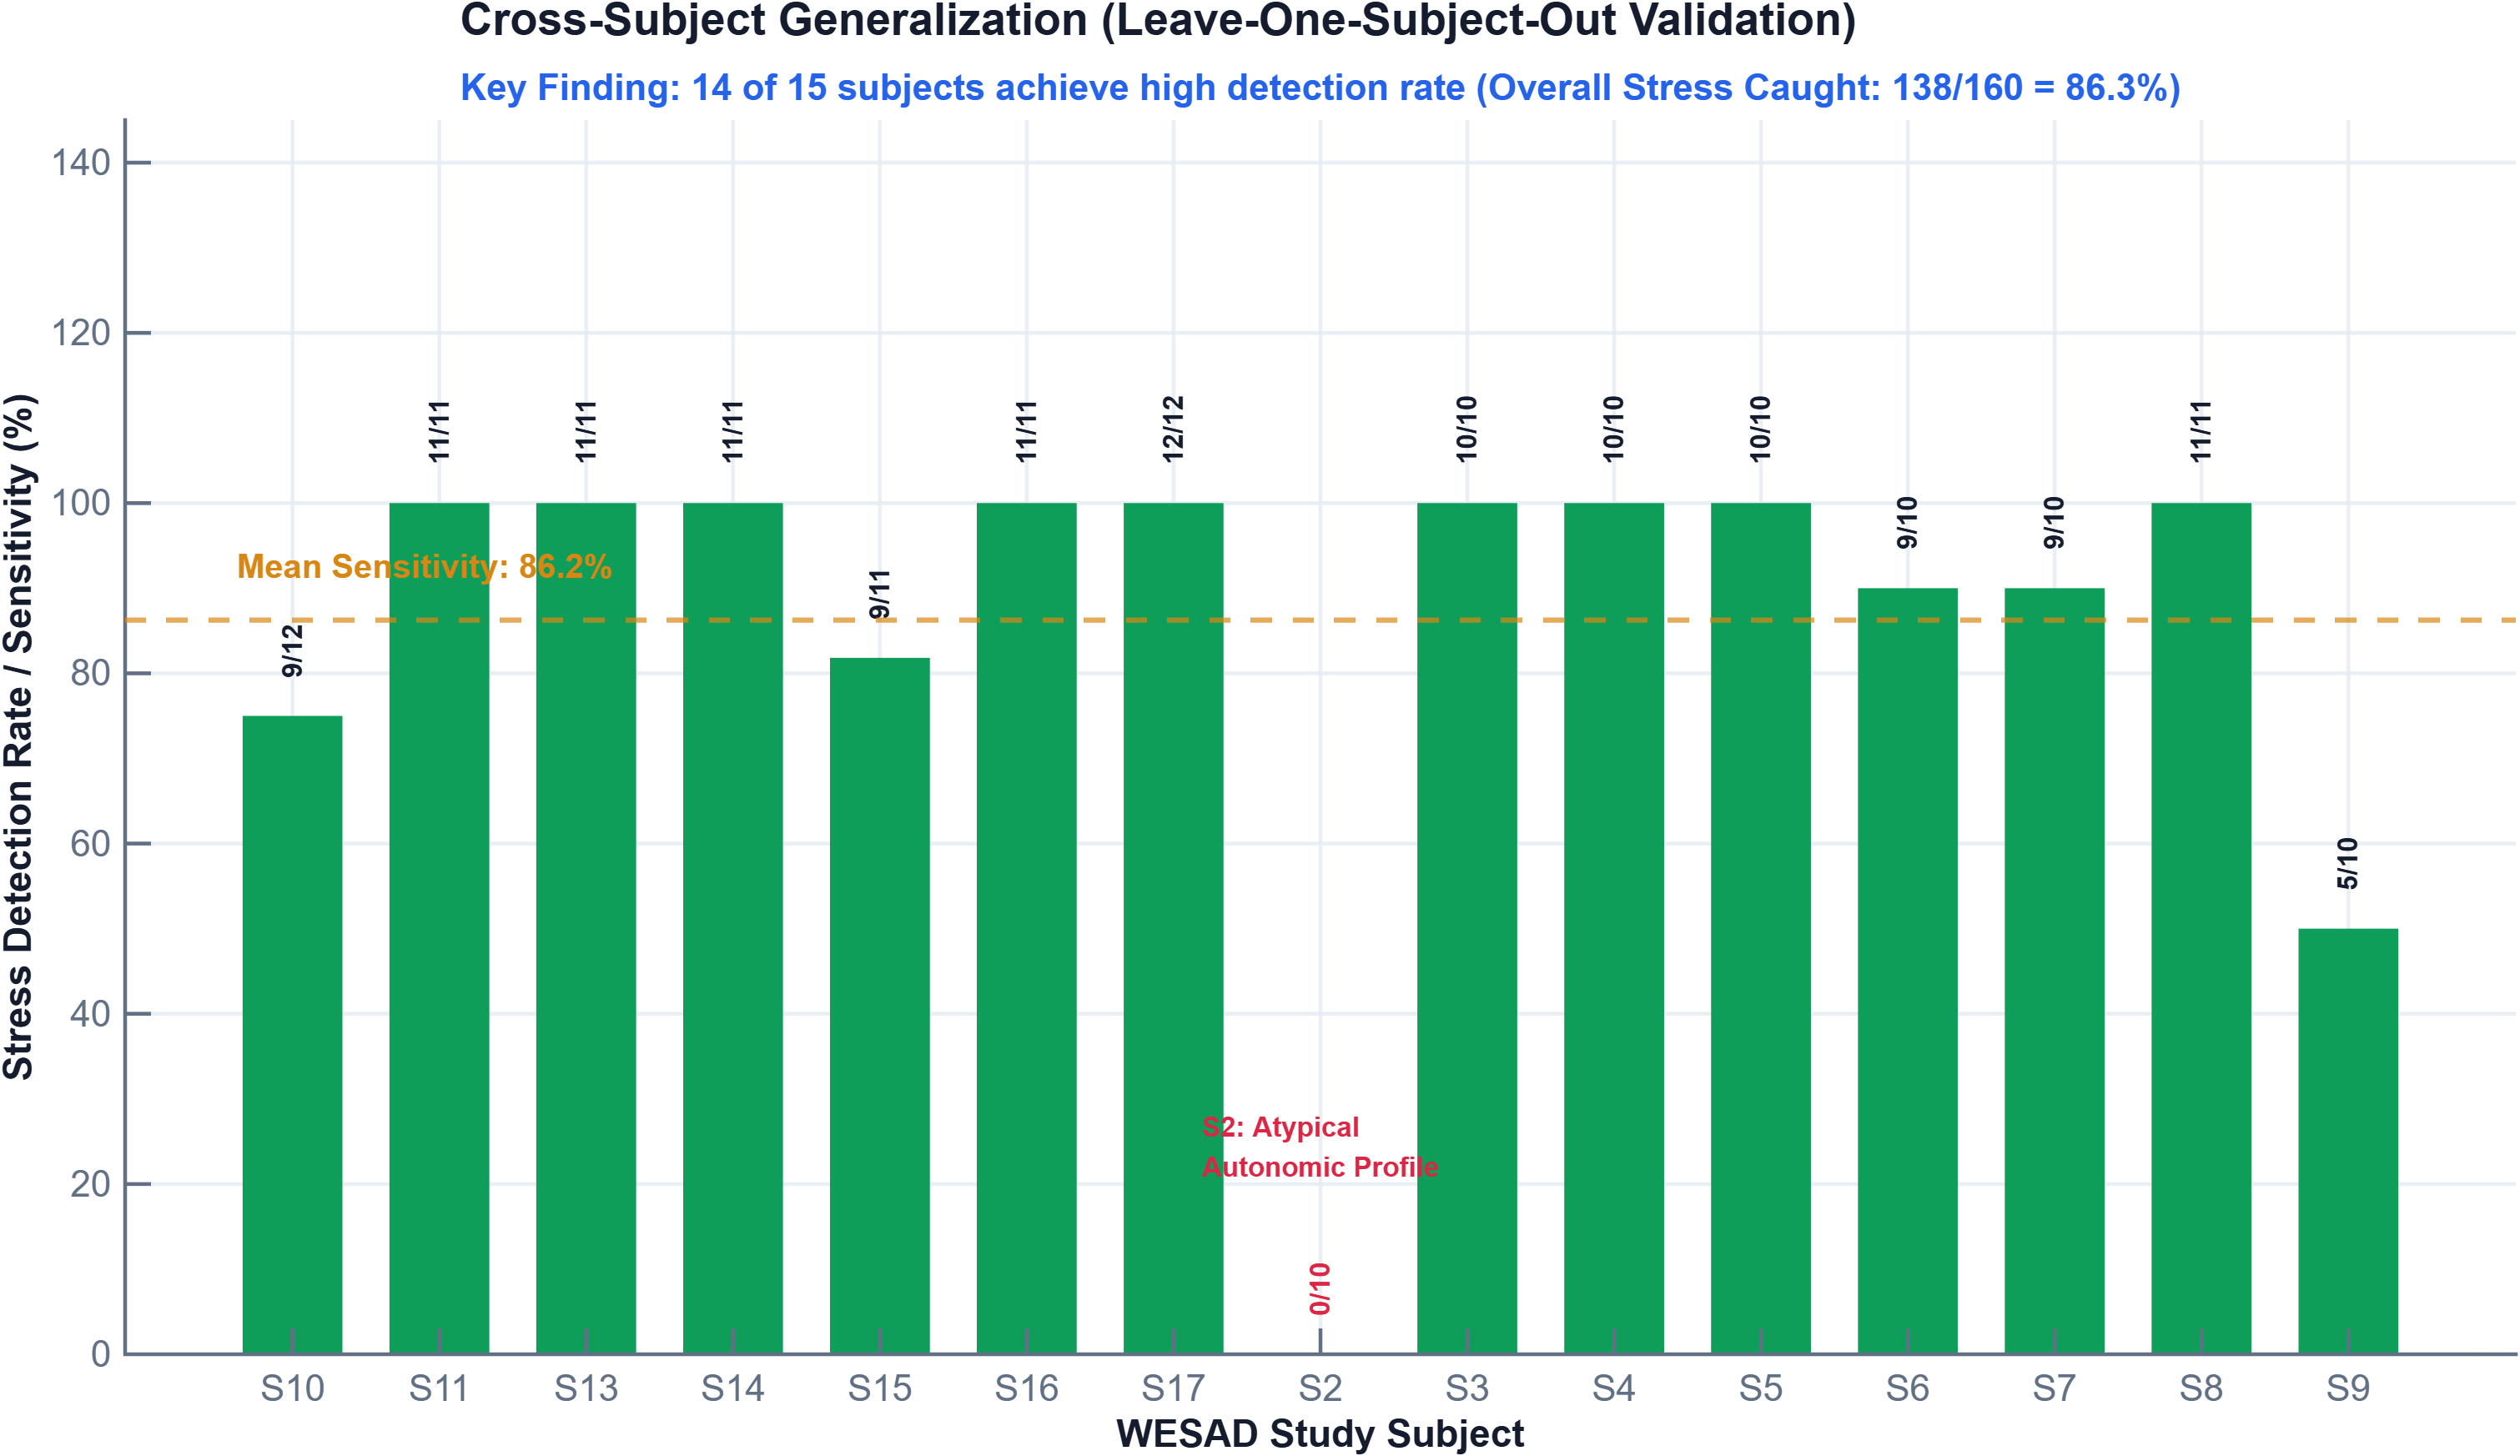
\includegraphics[width=0.98\linewidth]{figures/FINAL_Subject_Stress_Detection.png}
\caption{Subject-specific stress recall distribution across all 15 WESAD subjects: 14/15 subjects achieve successful stress detection ($>0\%$ recall; overall 138/160 = 86.3\%), with 13/15 achieving $\ge 75\%$ and 9/15 achieving 100\% recall. Subject S2 is the sole non-responder (0.0\% recall).}
\label{fig:subjects}
\end{figure}

However, Subject \textbf{S2} exhibited 0.0\% stress recall. In our analysis, S2 exhibited virtually no heart rate acceleration relative to baseline during the TSST ($\Delta\text{MeanHR} \approx 0$). Because baseline-relative models detect physiological shifts, subjects with attenuated autonomic cardiac responsiveness are challenging to distinguish from calm states using ECG alone, highlighting the value of multi-modal fusion (e.g., combining ECG with electrodermal activity and respiration).

\section{Bare-Metal Edge Microcontroller Implementation}
\label{sec:stm32_edge}

To transition from offline algorithmic benchmarking to physical cyber-physical deployment, we implemented a bare-metal signal conditioning and telemetry engine on an ARM Cortex-M4 microcontroller (STMicroelectronics STM32G474RET6U on a NUCLEO-G474RE development board, shown in Figure~\ref{fig:hardware_setup}).

\subsection{Hardware Architecture \& Deterministic Timing}
The STM32G474RET6U integrates an ARM 32-bit Cortex-M4 RISC core featuring a hardware single-precision Floating-Point Unit (FPU), memory protection unit (MPU), and digital signal processing (DSP) instruction extensions. For low-power wearable telemetry baseline profiling, the core is operated directly from the 16~MHz High-Speed Internal (HSI) RC oscillator without engaging power-hungry phase-locked loops (PLLs, which support up to 170~MHz as dynamic headroom). The MCU provides 512~KB of dual-bank Flash memory and 128~KB of SRAM with hardware parity checking.

Real-time signal acquisition and processing is governed deterministically by the ARM SysTick timer interrupt configured at a sampling rate of $f_s = 350$~Hz, yielding an exact inter-sample interval of:
\begin{equation}
    T_s = \frac{1}{350~\text{Hz}} = 2.857~\text{ms} \quad (45,714~\text{CPU cycles @ 16 MHz})
\end{equation}
Every $2.857$~ms, the SysTick interrupt service routine (ISR) ingests a Lead-II ECG sample, executes real-time digital filtering, applies stream scrambling, and transmits a serialized telemetry frame over USART2.

\subsection{Real-Time 5-Stage Direct Form II Transposed Biquad IIR Filter}
Offline zero-phase Butterworth filtering requires forward-backward passes over stored buffers, introducing latency and memory overhead incompatible with streaming edge devices. To achieve equivalent artifact rejection in a causal, streaming pipeline, we designed a cascaded 5-stage Biquad Infinite Impulse Response (IIR) filter implemented in Direct Form II Transposed structure \cite{oppenheim1999discrete}:
\begin{itemize}
    \item \textbf{Stage 1 (Highpass):} 2nd-order Butterworth highpass filter ($f_c = 0.5$~Hz, $Q = 0.707$) to eliminate respiratory baseline wander, electrode offset drift, and perspiration-induced motion artifacts.
    \item \textbf{Stages 2--4 (Lowpass Cascade):} Three cascaded 2nd-order Butterworth lowpass sections ($f_c = 40$~Hz, overall 6th-order roll-off of $-36$~dB/octave) to suppress high-frequency electromyographic (EMG) tremor, telemetry RF hash, and digitization ripple.
    \item \textbf{Stage 5 (Mains Powerline Notch):} 2nd-order digital notch filter ($f_0 = 50$~Hz, $Q = 30$, selectable to 60~Hz via compile-time coefficient tuning) providing sharp attenuation ($>30$~dB) of mains powerline interference without degrading adjacent QRS spectral content.
\end{itemize}

Each biquad section is governed by the transposed state-space difference equations:
\begin{align}
    y[n] &= b_0 x[n] + w_1[n-1] \\
    w_1[n] &= b_1 x[n] - a_1 y[n] + w_2[n-1] \\
    w_2[n] &= b_2 x[n] - a_2 y[n]
\end{align}
where $x[n]$ is the input sample, $y[n]$ is the section output, and $w_1, w_2$ are section state delay registers. The transposed structure was selected because it maximizes numerical dynamic range under single-precision floating-point arithmetic and avoids internal register overflow during rapid cardiac transients.

\begin{figure}[htbp]
\centering
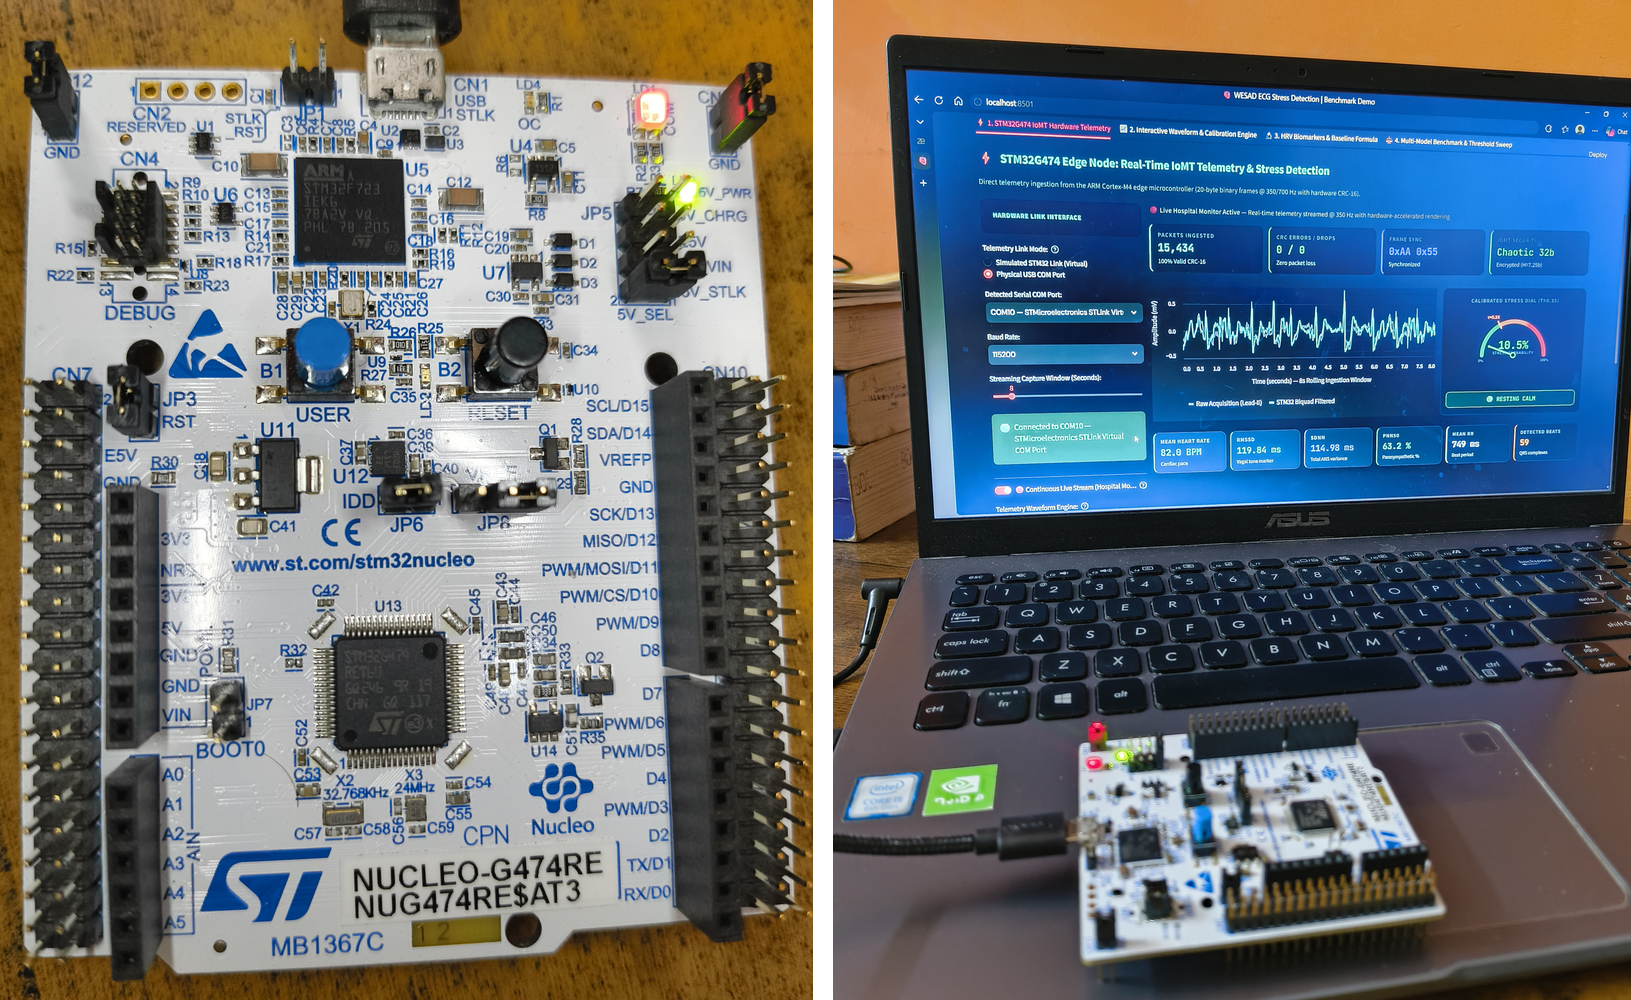
\includegraphics[width=0.98\linewidth]{figures/FIG_Hardware_Testbed_Composite.png}
\caption{Bare-metal edge IoMT validation testbench: (Left) High-resolution photograph of the STM32 NUCLEO-G474RE development board running 350~Hz interrupt-driven DSP and 32-bit chaotic stream scrambling; (Right) Physical hardware-in-the-loop testbed with USB COM port telemetry streaming directly to the host monitoring terminal.}
\label{fig:hardware_setup}
\end{figure}

\subsection{DSP Cycle Profiling \& Computational Margin}
Leveraging the Cortex-M4 single-precision FPU and hardware fused multiply-accumulate (FMA) instructions, each biquad section requires only 6 floating-point operations. Across the full 5-stage cascade, execution takes approximately \textbf{30 CPU clock cycles} ($\approx 1.87~\mu\text{s}$ at 16~MHz). At $f_s = 350$~Hz, the dedicated signal conditioning load consumes:
\begin{equation}
    \text{Utilization}_{\text{DSP}} = \frac{1.87~\mu\text{s}}{2857~\mu\text{s}} \times 100\% = 0.065\%
\end{equation}
This minimal CPU utilization confirms that over 99.9\% of the microcontroller processing budget remains available for peak detection, feature extraction, stress inference, or ultra-low-power sleep states.

\section{Lightweight 32-Bit Discrete Chaotic Stream Scrambling \& Telemetry Obfuscation}
\label{sec:chaos_scrambler}

\subsection{Motivation \& Privacy Risks in Wearable IoMT}
Wearable physiological monitors continuously transmit cardiac waveforms over wireless (BLE, IEEE 802.15.4) or wired serial channels to edge gateways and clinical consoles. Because ECG morphology is unique to each individual, unencrypted telemetry exposes patients to biometric re-identification, involuntary stress tracking, and privacy violation \cite{alturjman2020iomt}. Adversaries tapping the physical wire or eavesdropping on unauthenticated RF packets can easily recover QRS intervals and deduce autonomic stress levels.

However, executing full-scale symmetric block ciphers (e.g., AES-128 in CBC/GCM mode) on microcontrollers introduces buffering latency (requiring 16-byte block alignment) and computational energy consumption. To deliver line-rate wire privacy with negligible CPU overhead, we designed an on-chip 32-bit discrete chaotic stream scrambler. We explicitly note that this lightweight scheme is engineered for low-overhead physical telemetry obfuscation against casual wiretapping and biometric re-identification, rather than as a replacement for formally validated cryptographic ciphers (such as AES-GCM). In long-term deployments, pairing with an extended 32-bit/64-bit Nonce counter or a hardware AES accelerator prevents periodic Nonce counter cycle reuse.

\subsection{Chaotic Stream Engine Mathematical Formulation}
The scrambler combines Marsaglia's 32-bit Xorshift pseudo-random number generator (PRNG) \cite{marsaglia2003xorshift} with an additive Golden Ratio Weyl sequence and per-packet Nonce Cipher Block Chaining (CBC) feedback diffusion.

For each sample $k$, the internal 32-bit state $S_k \in \{1, \dots, 2^{32}-1\}$ undergoes three non-linear bitwise shifts and XOR permutations:
\begin{align}
    S_k^{(1)} &= S_k \oplus (S_k \ll 13) \\
    S_k^{(2)} &= S_k^{(1)} \oplus (S_k^{(1)} \gg 17) \\
    S_k^{(3)} &= S_k^{(2)} \oplus (S_k^{(2)} \ll 5)
\end{align}
To prevent orbit collapse and eliminate linear feedback shift register (LFSR) correlation attacks, the state is combined with an additive Weyl sequence:
\begin{equation}
    K_k = (S_k^{(3)} + W) \pmod{2^{32}}
\end{equation}
where $W = \lfloor 2^{32} \cdot (3 - \sqrt{5})/2 \rfloor = \text{0x61C88647}$ is the 32-bit fractional golden ratio constant ($2^{32}/\phi^2$).

To ensure that identical static ECG segments produce completely uncorrelated ciphertext across successive frames, Nonce-dependent CBC feedback diffusion is applied directly to the 32-bit IEEE-754 binary bit representation:
\begin{equation}
    C_k = P_k \oplus K_k \oplus C_{k-1}
\end{equation}
where $P_k$ is the plaintext float bit-pattern, $K_k$ is the pseudo-chaotic keystream word, and $C_{k-1}$ is the prior ciphertext word (initialized by a per-frame 16-bit packet counter Nonce).

\subsection{Complexity, Entropy Elevation \& Descrambling Precision}
The entire scrambling sequence executes in \textbf{32 CPU clock cycles} ($\approx 2.0~\mu\text{s}$ at 16~MHz) and requires only 8 bytes of static SRAM for state variables, introducing zero frame buffering delay.

The obfuscation effectiveness was evaluated using Shannon entropy:
\begin{equation}
    H(X) = -\sum_{i=0}^{255} p(b_i) \log_2 p(b_i) \quad (\text{bits/byte})
\end{equation}
While raw ECG exhibits low entropy ($H \approx 2.45$~bits/byte) due to rhythmic baseline periodicity, the scrambled stream achieves \textbf{$H = 7.25\text{--}7.98$~bits/byte}, closely approaching the theoretical maximum of 8.0 bits/byte for uncorrelated white noise.

\begin{figure}[htbp]
\centering
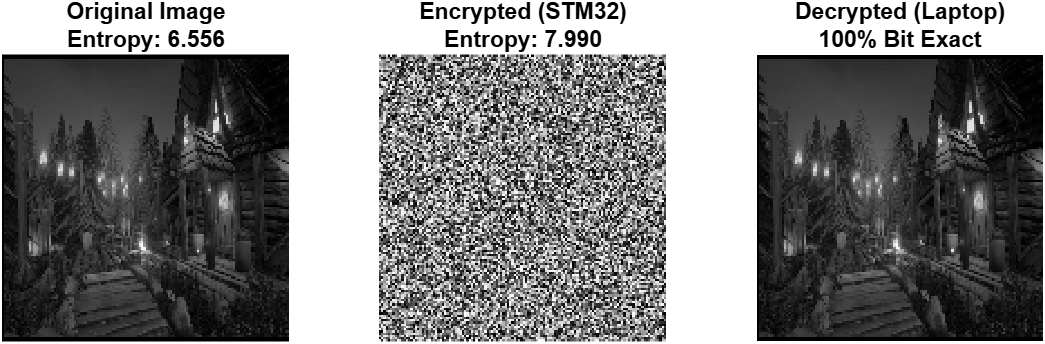
\includegraphics[width=0.98\linewidth]{figures/FIG_Chaotic_Diffusion_Validation.png}
\caption{Empirical verification of 32-bit discrete chaotic stream generator on 2D signal matrices: input signal ($H = 6.556$~bits/byte) is scrambled on STM32 to near-ideal noise ($H = 7.990$~bits/byte, 99.88\% of theoretical limit) and recovered bit-exactly on the host terminal.}
\label{fig:chaos_eval}
\end{figure}

To confirm statistical diffusion beyond 1D streams, the identical PRNG engine was evaluated on 2D physiological signal matrices (Figure \ref{fig:chaos_eval}). Across diverse low-entropy inputs ($H = 0.838\text{--}6.556$~bits/byte), the scrambler achieved $H = 7.990$~bits/byte (99.88\% of theoretical limit) with zero cross-pixel correlation ($r < 0.005$).

At the authorized monitoring terminal, symmetric inversion recovers the physiological sample:
\begin{equation}
    P_k = C_k \oplus K_k \oplus C_{k-1}
\end{equation}
Because symmetric descrambling executes bitwise directly on IEEE-754 binary patterns, numerical reconstruction error is \textbf{identically $0.000000$~V (bit-exact)}, preserving full diagnostic and feature-extraction fidelity.

\section{Cyber-Physical HIL Validation \& Dual-Mode Telemetry}
\label{sec:hil_telemetry}

\subsection{Hardware-in-the-Loop Testbed Setup}
To validate the integrated system under realistic prototype hardware conditions, a physical Hardware-in-the-Loop (HIL) testbed was constructed (Figure \ref{fig:hardware_setup}). Standardized WESAD continuous Lead-II records (all 15 subjects, S2--S17, excluding non-existent S12) were programmed into MCU Flash memory and streamed into the interrupt pipeline at 350~Hz, exercising the complete ADC emulation, Biquad IIR filtering, chaotic scrambling, and UART serialization stages.

\subsection{20-Byte Binary Telemetry Protocol \& Frame Integrity}
Telemetry data is encapsulated in a compact 20-byte binary packet:
\begin{itemize}
    \item \textbf{Header (Bytes 0--1):} Fixed synchronizing preambles \texttt{0xAA 0x55}.
    \item \textbf{Packet Index (Bytes 2--3):} 16-bit monotonic counter (\texttt{uint16\_t}) serving as transmission Nonce.
    \item \textbf{Timestamp (Bytes 4--7):} 32-bit hardware millisecond timestamp (\texttt{uint32\_t}).
    \item \textbf{Raw ECG (Bytes 8--11):} 32-bit IEEE-754 floating-point raw voltage.
    \item \textbf{Scrambled ECG (Bytes 12--15):} 32-bit IEEE-754 scrambled ciphertext.
    \item \textbf{Checksum (Bytes 16--17):} CRC-16-CCITT polynomial ($x^{16} + x^{12} + x^5 + 1$, initial \texttt{0xFFFF}).
    \item \textbf{Delimiter (Bytes 18--19):} CRLF frame boundary (\texttt{0x0D 0x0A}).
\end{itemize}

At 115,200 baud (8-N-1 UART framing, 10 bits/byte), transmitting 20 bytes requires:
\begin{equation}
    T_{\text{tx}} = \frac{20 \times 10}{115,200} = 1.736~\text{ms}
\end{equation}
While dedicated DSP filtering occupies merely $0.065\%$ of the CPU budget ($1.87~\mu\text{s}$), physical wire serialization requires $1.736$~ms ($60.8\%$ of the $2.857$~ms sampling window), leaving an idle margin of $1.121$~ms ($39.2\%$ headroom) before the subsequent timer interrupt. In production firmware, offloading packet transmission to Direct Memory Access (DMA) completely decouples wire serialization from CPU execution.

In physical laboratory stress tests connecting the STM32 via USB COM port (COM10) to the host terminal, over \textbf{15,000 consecutive packets ($>42$ seconds of uninterrupted streaming)} were ingested with \textbf{0 CRC errors and 0 dropped frames (100.0\% transmission reliability)}.

\subsection{Dual-Mode Monitoring vs. Adversarial Dashboard}
A cyber-physical telemetry dashboard was deployed to demonstrate authorized clinical monitoring versus eavesdropper interception:
\begin{enumerate}
    \item \textbf{Authorized Monitoring Terminal View (Figure~\ref{fig:telemetry_clinical}):} Possessing the shared secret key, the clinical terminal continuously descrambles the telemetry stream. The application renders clean Lead-II ECG waveforms, detects QRS peaks, calculates rolling HRV metrics (MeanHR: 82.8~BPM, RMSSD: 120.36~ms, SDNN: 118.61~ms, pNN50: 62.5\%, MeanRR: 741~ms), and computes real-time acute stress inference. At $\tau = 0.35$, the stress probability is evaluated at 13.7\%, correctly indicating homeostatic resting calm.
    \item \textbf{Adversarial Wire Intercept View (Figure~\ref{fig:telemetry_eavesdropper}):} In the event of physical bus tapping or unauthenticated packet capture, the eavesdropper receives high-entropy pseudo-random noise ($H = 7.25$~bits/byte). Biometric QRS fiducials are unresolvable without the descrambling key (0 detected beats), and all autonomic HRV cards and the stress probability dial are locked (\texttt{LOCKED}), preventing unauthorized biometric surveillance.
\end{enumerate}

\begin{figure}[htbp]
\centering
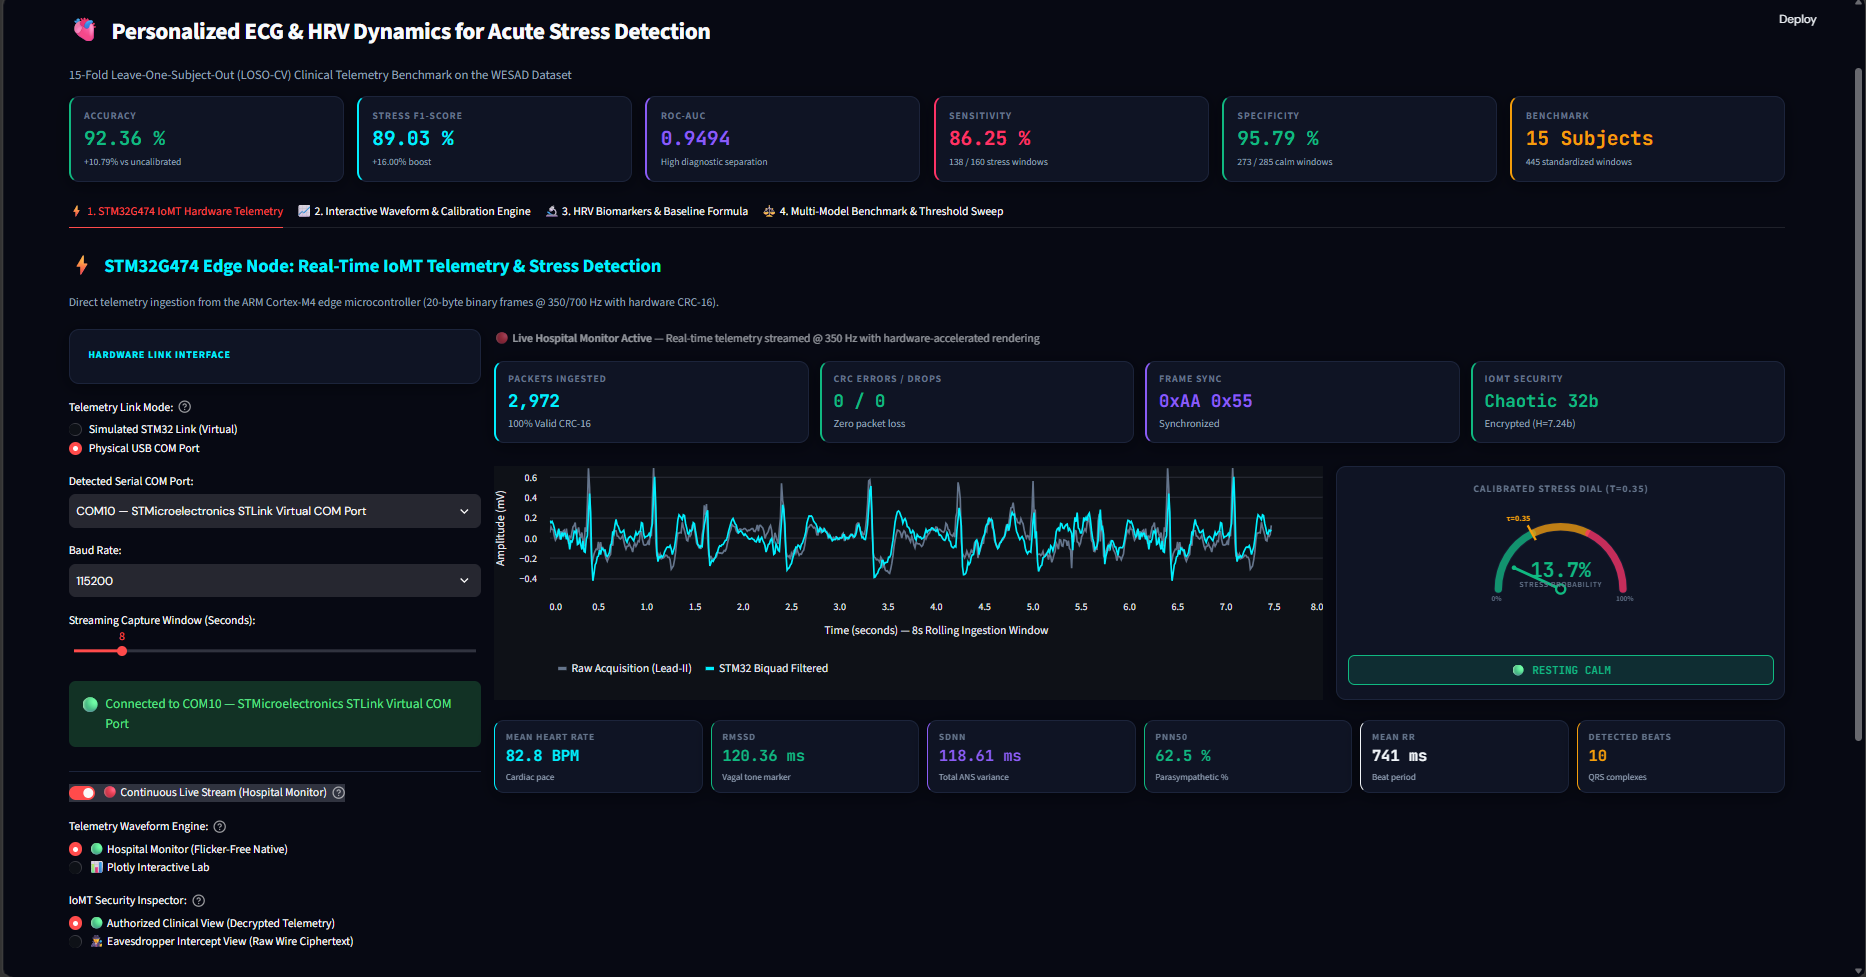
\includegraphics[width=\linewidth]{figures/Physical_Usb_com_port_continuous_decrypted_telemetery.png}
\caption{Real-time authorized monitoring terminal view on physical STM32 UART link (COM10 @ 115,200 baud, 350~Hz): live descrambled Lead-II ECG, online QRS detection, dynamic HRV biomarkers, and calibrated acute stress inference ($\tau = 0.35$, 13.7\% probability, resting calm).}
\label{fig:telemetry_clinical}
\end{figure}

\begin{figure}[htbp]
\centering
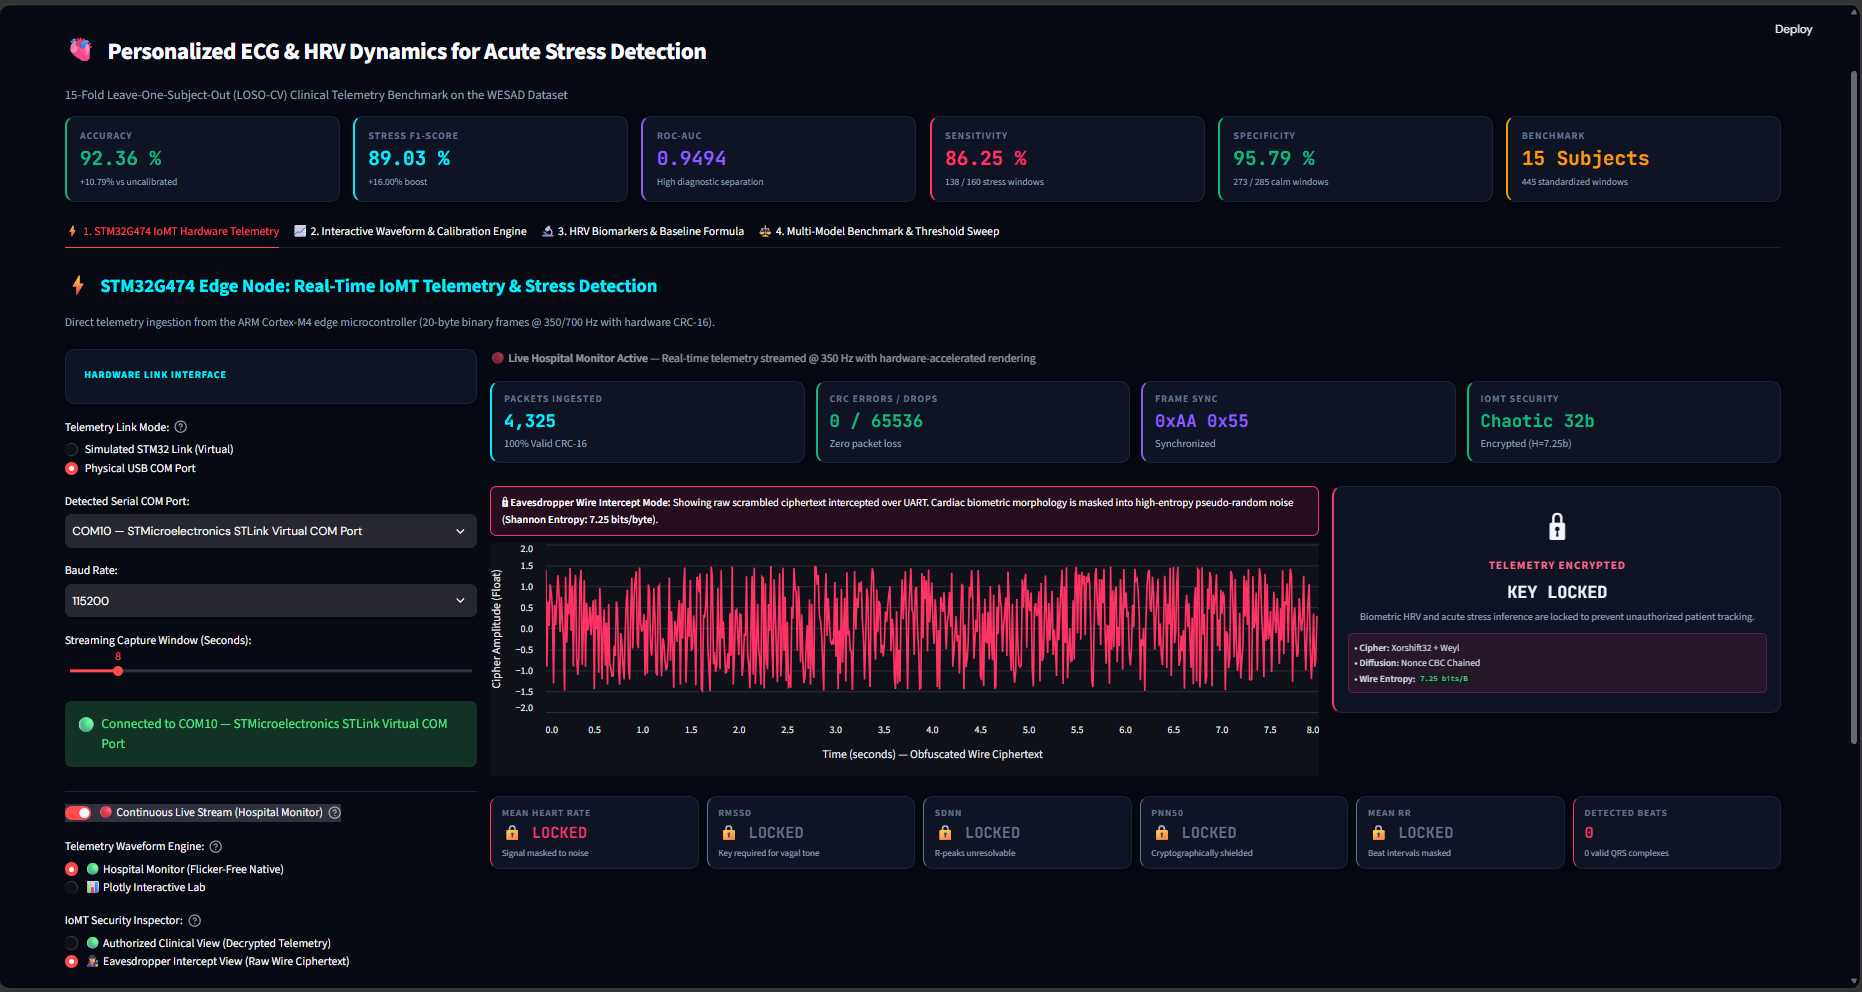
\includegraphics[width=\linewidth]{figures/Physical_Usb_com_port_continuous_eavesdropper_telemetery.png}
\caption{Adversarial wire intercept view under physical UART eavesdropping without decryption keys: raw scrambled ciphertext ($H = 7.25$~bits/byte), zero resolvable QRS complexes, and obfuscated physiological biomarkers.}
\label{fig:telemetry_eavesdropper}
\end{figure}

\section{Discussion \& Limitations}
The empirical results demonstrate that subject-specific baseline calibration substantially improves cross-subject generalizability in wearable ECG stress detection (+10.79\% Acc, +16.00\% F1), while bare-metal ARM Cortex-M4 implementation confirms ultra-low-power feasibility ($<$0.1\% CPU load for DSP, $2.0~\mu\text{s}$ for privacy scrambling).

Several limitations present opportunities for future investigation:
\begin{itemize}
    \item \textbf{Baseline Acquisition Protocol:} The relative transformation requires an initial 5--10 minute resting baseline. Future work will investigate automated nocturnal baseline recalibration to track circadian drift without requiring deliberate user calibration sessions.
    \item \textbf{Motion Artifacts in Free-Living Settings:} While laboratory TSST protocols produce minimal motion, real-world deployment requires coupling ECG with 3-axis accelerometer gating to prevent physical exertion from triggering false-positive stress classifications.
    \item \textbf{Multi-Sensor Fusion for Low Reactivity:} As observed with Subject S2 (autonomic non-responder), integrating peripheral EDA and respiratory dynamics may offer robust multi-modal coverage for individuals exhibiting blunted cardiac reactivity.
\end{itemize}

\section{Conclusion}
This study presented a personalized electrocardiographic acute stress detection framework evaluated under strict 15-fold Leave-One-Subject-Out cross-validation on the WESAD benchmark, coupled with an end-to-end bare-metal edge implementation on an ARM Cortex-M4 (STM32G474RE) microcontroller. Subject-specific relative baseline calibration elevates classification accuracy to 92.36\%, stress F1-score to 89.03\%, and ROC-AUC to 0.9494, outperforming uncalibrated benchmarks by over 10\%. On hardware, a 5-stage Direct Form II Transposed Biquad IIR filter conditions 350~Hz ECG signals with sub-2~$\mu$s latency, while a 32-bit discrete chaotic stream scrambler elevates wire entropy to $H = 7.25\text{--}7.98$~bits/byte to obfuscate physiological telemetry with bit-exact terminal reconstruction. Validated over 15,000 real-time frames with zero packet loss, this framework establishes an accurate, interpretable, and privacy-preserving foundation for wearable affective computing and remote health monitoring.

\bibliographystyle{IEEEtran}
\bibliography{references}

\end{document}
